\documentclass[11pt]{article}
% Suppress the output-path-dependent pdfTeX trailer identifier.
% SOURCE_DATE_EPOCH fixes the metadata dates for portable byte reproduction.
\pdftrailerid{}
\pdfminorversion=7 % Match the version of the retained PDF figure assets.
\usepackage[T1]{fontenc}
\usepackage{lmodern}
\usepackage{amsmath,amssymb,amsthm,mathtools,mathrsfs}
\usepackage[a4paper,margin=27mm]{geometry}
\usepackage{microtype,booktabs,array,graphicx,placeins,flafter}
\usepackage{tikz}
\usetikzlibrary{arrows.meta,calc,positioning}
\usepackage[colorlinks=true,linkcolor=blue!45!black,citecolor=blue!45!black,urlcolor=blue!45!black]{hyperref}
\urlstyle{same}
\hypersetup{pdftitle={Cyclicity Six and Saturation Geometry at Cancelling Double Grazing},pdfauthor={Haibo Lu}}
\usepackage[nameinlink,noabbrev]{cleveref}
\newtheorem{theorem}{Theorem}[section]
\newtheorem{proposition}[theorem]{Proposition}
\newtheorem{lemma}[theorem]{Lemma}
\newtheorem{corollary}[theorem]{Corollary}
\theoremstyle{definition}
\newtheorem{definition}[theorem]{Definition}
\theoremstyle{remark}
\newtheorem{remark}[theorem]{Remark}
\numberwithin{equation}{section}
\newcommand{\R}{\mathbb R}
\newcommand{\sgn}{\operatorname{sgn}}
\newcommand{\id}{\operatorname{id}}
\newcommand{\Fl}{\operatorname{Fl}}
\newcommand{\eps}{\varepsilon}
\newcommand{\bsc}{\beta_4}
\newcommand{\dsc}{d_4}
\newcommand{\smallO}{\mathrm{o}}
\newcommand{\bigO}{\mathrm{O}}
\title{Cyclicity Six and Saturation Geometry\\at Cancelling Double Grazing}
\author{Haibo Lu\\[2pt]
\small Shanghai Institute of Technology, Shanghai 201418, China\\
\small Corresponding author: \href{mailto:luhaibo1985@gmail.com}{luhaibo1985@gmail.com}\\
\small ORCID: \href{https://orcid.org/0009-0000-2717-5968}{0009-0000-2717-5968}}
\date{}
\begin{document}
\maketitle
\begin{abstract}
We determine the sharp cyclicity of a semistable limit cycle with two
separated quadratic grazings in a continuous piecewise smooth planar system.
The active sides agree under transverse transport, two nonzero passage
strengths cancel, and the smooth closing curvature is nonzero. The reference
displacement is $C^2$ with an ordinary double zero, yet the cyclicity is six.
Changes in the strength sum and activation thresholds prevent joint $C^2$
regularity of the unfolding.

An exact curvature-zero graph and threshold estimates give this upper bound
in every fixed admissible family preserving the prescribed grazing geometry,
at arbitrary relative rates of four controls: closing offset, multiplier
defect, strength sum and threshold separation. The bounds are four when the
strength sum vanishes or the thresholds align, and two when both hold.
Full-rank unfoldings attain all four bounds. Six-cycle configurations force
weighted bounds on the controls and cycle locations. For positive first
passage strength and negative closing curvature, the closures of the
rescaled six-cycle domains in a fixed full-rank unfolding converge in
Hausdorff distance to a quartic coefficient region with four nonnegative
roots, counted with multiplicity.

In this sign case, a fourfold boundary root continues to a cycle of
multiplicity four for every small positive strength sum. With two simple
companion cycles, its local unfolding gives complete counts of two, four or
six simple cycles on the common return interval, off the multiple-root set.
A predator--prey model with continuous threshold harvesting realizes the
four controls through its natural parameters.
\end{abstract}
\noindent\textbf{Keywords.} Continuous piecewise smooth planar systems;
grazing bifurcation; cyclicity; Poincar\'e return maps;
multiple limit cycles.
\par\smallskip
\noindent\textbf{Mathematics Subject Classification.}
Primary 34C23; Secondary 34A36, 34C25, 37G15.
\par\smallskip
\section{Introduction and main results}\label{sec:introduction}

In a jointly $C^2$ unfolding, a periodic orbit whose return displacement
has an ordinary double zero has at most two nearby cycles: the second
derivative keeps its sign, and Rolle's theorem applies~\cite{roussarie1998}.
We study a continuous piecewise smooth planar system in which the reference
displacement has such a double zero, but the sharp local cyclicity is six.

The reference orbit has two spatially separated quadratic grazings, with both
active sides agreeing after transport to one transverse section. Each
passage contributes a term of order $q^{3/2}$ in a transported transverse
coordinate $q$~\cite{dibbc2001,nordmark2002}, and their nonzero leading
coefficients cancel. The quadratic defect of the composed passages cancels
as well, as the expansion below shows. The reference displacement is therefore $C^2$, with
its nonzero quadratic term supplied by the smooth closing map. Under
perturbation, the strength sum can become nonzero and the activation
thresholds can separate, so the family need not be jointly $C^2$.
Together with the closing offset and multiplier defect, these give four
scalar return-map controls. We answer three questions.
\begin{enumerate}
\item[(Q1)] What is the cyclicity of the reference cycle?
\item[(Q2)] What parameter scales are necessary for six limit cycles,
and what is the limiting shape of the six-cycle parameter set?
\item[(Q3)] Does a fourfold root of the limiting polynomial continue
to a cycle of multiplicity four, and what is its local unfolding?
\end{enumerate}
Theorems~\ref{thm:six-main}, \ref{thm:main-saturation-summary}
and~\ref{thm:actual-quartic-summary} below answer these questions.

\subsection{The return map}

In each of the two grazing boxes, the planar equation has the local form
\[
 \dot{\mathbf{x}}=X^-_\lambda(\mathbf{x})
 +(h_\lambda(\mathbf{x}))_+Z_\lambda(\mathbf{x}),
 \qquad \mathbf{x}\in\R^2,\qquad u_+=\max\{u,0\}.
\]
The local data are jointly smooth in state and parameters and may differ
between the boxes. The active branch
$X^+_\lambda=X^-_\lambda+h_\lambda Z_\lambda$ agrees with $X^-_\lambda$
on the seam $\{h_\lambda=0\}$, so the field is continuous there.
The boxes are joined by regular flow arcs; Definition~\ref{def:admissible-family}
gives the precise admissibility conditions. The threshold-harvesting family
of Theorem~\ref{thm:harvesting-realization} realizes these conditions.

In a transverse coordinate $q$ constructed in Section~\ref{sec:passage}, the
return map and the displacement have the form
\[
 P(q)=R\{\delta+\Gamma_2(\Gamma_1(q)-\delta)\},
 \qquad D(q)=P(q)-q.
\]
Here $\Gamma_1,\Gamma_2$ are the passage maps near the two tangencies, $R$ is
the smooth transition along the rest of the cycle, and parameter dependence is
suppressed. The second passage is activated by the intermediate input
$\Gamma_1(q)-\delta$, so the two grazing thresholds on the section are $0$ and
$\Gamma_1^{-1}(\delta)$. Section~\ref{sec:passage} derives this composition
from the vector field and shows that it is the first return on a fixed
interval.

We use four return-map controls,
\[
 a=R(0),\qquad b=R'(0)-1,\qquad m=A_1+A_2,\qquad\delta,
\]
namely the offset, the multiplier defect, the strength sum and the threshold
separation. They are smooth functions of the physical parameters and need not
be independent. All four vanish at the reference parameter, where $A_1=-A_2\ne0$
and $c_0=R''(0)/2\ne0$. Writing $q_+=\max\{q,0\}$, the correction
$\Gamma_\nu(q)-q$ begins with $A_\nu q_+^{3/2}$, and the reversibility of the
quadratic passage fixes its next coefficient at $3A_\nu^2/4$
(Proposition~\ref{prop:quadratic-passage}). Consequently, when the thresholds
are aligned,
\[
 \Gamma_2(\Gamma_1(q))-q
 =mq_+^{3/2}+\tfrac34m^2q_+^2+O(q_+^{5/2})
 \qquad(\delta=0).
\]
Both displayed terms vanish when $m=0$, so the quadratic term of the reference
displacement comes from $R$ (Lemma~\ref{lem:passage:finite-inverse}). For
$\delta\ne0$, the two $q^{3/2}$ contributions start at different thresholds.
Their singular curvatures have opposite signs and compete. Neither an outer
expansion nor the number of active intervals controls the fixed-point count
on the whole return interval; estimates relative to the moving thresholds
are needed.

We use the standard notion of cyclicity~\cite{roussarie1998}.

\begin{definition}[Cyclicity]\label{def:cyclicity}
Let $(X_\lambda)$ be a family of planar vector fields and let $\mathcal C$ be a
periodic orbit of $X_{\lambda_0}$. Let $N(\lambda,\varepsilon)$ be the number
of limit cycles of $X_\lambda$ at Hausdorff distance less than $\varepsilon$
from $\mathcal C$. The cyclicity of $\mathcal C$ in $(X_\lambda)$ is
\[
 \operatorname{Cycl}\bigl((X_\lambda),\mathcal C\bigr)
=\inf_{\varepsilon,\eta>0}\ \sup_{|\lambda-\lambda_0|<\eta}N(\lambda,\varepsilon).
\]
For a class $\mathfrak F$ of families through
$X_{\lambda_0}$, $\operatorname{Cycl}(\mathfrak F,\mathcal C)$ denotes the supremum
over the families in $\mathfrak F$.
\end{definition}

The families we consider are the admissible families of
Definition~\ref{def:admissible-family}: finite-dimensional smooth families of
continuously matched fields that preserve regular switching curves, the two
quadratic tangencies, their transported active side and the one-turn itinerary
of $\mathcal C$, with
$a=b=\delta=0$, $A_1=-A_2\ne0$ and $c_0\ne0$ at the reference parameter.
When the map $\lambda\mapsto(a,b,m,\delta)$ is a submersion at
$\lambda_0$, we fix a local inverse
\[
 \Lambda(a,b,m,\delta)=\lambda(a,b,m,\delta;\xi_0),
\]
with the remaining parameters fixed at $\xi_0$, and call the resulting
fixed four-parameter family the \emph{standard unfolding}.

\subsection{Sharp cyclicity}

\begin{theorem}[Cyclicity]\label{thm:six-main}
Let $\mathfrak F$ be the class of admissible families through the reference
field.
\begin{enumerate}
\item For every family in $\mathfrak F$ there are a neighbourhood $U$ of
$\lambda_0$ and an interval $I=(-q_0,q_0)$ on the transverse section such
that, for every $\lambda\in U$, the return map $P_\lambda$ has at most six
fixed points in $I$; at most four if $m(\lambda)=0$ or $\delta(\lambda)=0$;
and at most two if $m(\lambda)=\delta(\lambda)=0$.
\item If $\lambda\mapsto(a,b,m,\delta)$ is a submersion at $\lambda_0$,
all four bounds are attained by hyperbolic fixed points along smooth
parameter paths in the corresponding slices that tend to $\lambda_0$.
For every sufficiently small $m$ with $mc_0<0$, the standard unfolding
has six hyperbolic fixed points of order $m^2$ in $I$ whenever
$(a/m^4,b/m^2,\delta/m^3)$ belongs to a fixed nonempty open set.
Three cycles are attracting and three repelling.
\item Consequently $\operatorname{Cycl}(\mathfrak F,\mathcal C)=6$. The
corresponding suprema over admissible families contained in $\{m=0\}$, in
$\{\delta=0\}$ and in $\{m=\delta=0\}$ are four, four and two.
\end{enumerate}
\end{theorem}

The proof controls curvature before counting fixed points. With the other
controls fixed, the outer equation $P''(q)=0$ is represented exactly by a
separation graph $\delta=\Delta(r)$, $r=\sqrt q$. This graph has at most one
positive critical point, and hence at most two intersections with a fixed
separation level. Estimates relative to the moving thresholds exclude
further curvature zeros outside the outer region. The two possible
curvature zeros and the two thresholds divide the continuous derivative
$P'$ into at most five strictly monotone pieces. Thus $P'-1$ has at most
five zeros, and Rolle's theorem gives at most six fixed points, including
those at the thresholds.

Theorem~\ref{thm:six-main} is proved in Section~\ref{sec:curvature-graph}
(Proposition~\ref{prop:common-count}, Corollary~\ref{cor:four-slices} and
Propositions~\ref{prop:single-scale-six}--\ref{prop:sharp-slice-attainment})
and Section~\ref{subsec:specified-field}. Proposition~\ref{prop:specified-rank}
constructs, through every reference field, an admissible family for which
$\lambda\mapsto(a,b,m,\delta)$ is a submersion; Corollary~\ref{cor:specified-cyclicity}
gives the same cyclicity in the smaller class of local perturbations used there.

\subsection{The saturation domain}

For an admissible family we call the set of parameters $\lambda\in U$ for
which $P_\lambda$ has six fixed points in $I$ the \emph{saturation domain},
and a sequence of such parameters tending to $\lambda_0$ a \emph{saturated
sequence}. Describing this set requires estimates that remain valid when the
parameters tend to the reference at arbitrary relative rates, including
configurations whose fixed points approach the thresholds. Six zeros of $D$
force five alternating extrema, and their locations and values constrain the
parameters.

Consider the sign case $A_1(\lambda_0)=B>0$, $c_0=-C<0$. Saturation forces
$m>0$, $\delta>0$ and $b<0$. Beyond both thresholds, the balance of
$mq^{3/2}$ and $-Cq^2$ suggests $q$ of order $m^2$. At this scale, $bq$, the
separation term $\tfrac32B\delta\sqrt q$ and the offset $a$ have the same order
when $b,\delta,a$ have weights $2,3,4$ relative to $m$.
Theorem~\ref{thm:main-saturation-summary} shows that every six-cycle
configuration obeys upper bounds with these weights.

Define the normalized parameters and the normalized positive state by
\[
 A_4=\frac{C^3a}{m^4},\qquad S_4=-\frac{Cb}{m^2},\qquad
 T_4=\frac{3BC^2\delta}{2m^3},\qquad x=\frac{C\sqrt q}{m}.
\]
The limiting polynomial is
\[
 \Phi_{A,S,T}(x)=A-Sx^2+x^3-x^4+Tx.
\]
With $e_j$ denoting the elementary symmetric polynomials of
$r=(r_1,r_2,r_3,r_4)$, set
\[
 \mathcal K_4=
 \left\{(-e_4(r),e_2(r),e_3(r)):
 r_i\ge0,\ \sum_{i=1}^4r_i=1\right\}.
\]
This is the compact set of coefficients for which $\Phi_{A,S,T}$ has four
nonnegative real roots, counted with multiplicity. For the standard unfolding
and $m>0$, let $\mathscr T_m$ be the set of $(A,S,T)$ in a fixed compact box
$\mathcal B$ for which the parameters
$(a,b,m,\delta)=(m^4A/C^3,\,-m^2S/C,\,m,\,2m^3T/(3BC^2))$ give six fixed points
in $I$; the box $\mathcal B$ contains all normalized six-cycle parameters
(see~\eqref{def:actual-main-domain}). We write $d_H$ for the Hausdorff distance
in $\R^3$.

\begin{theorem}[Saturation at the principal scale]\label{thm:main-saturation-summary}
\label{thm:k4-domain}
\begin{enumerate}
\item For every admissible family, after shrinking $U$ and $I$ if necessary,
there is $K>0$ such that, whenever
$\lambda\in U$ and $P_\lambda$ has six fixed points $q_1,\dots,q_6$ in $I$,
\[
 0<|\delta|\le K|m|^3,\quad |b|\le K|m|^2,
 \quad |a|\le K|m|^4,\quad \max_j|q_j|\le K|m|^2.
\]
\item For every admissible family in the sign case $A_1(\lambda_0)=B>0$,
$c_0=-C<0$, every accumulation point of $(A_4,S_4,T_4)$ along a saturated
sequence belongs to $\mathcal K_4$.
\item In the same sign case, for the standard unfolding,
\[
 d_H(\overline{\mathscr T_m},\mathcal K_4)\longrightarrow0\quad(m\to0^+).
\]
For every compact set $E\subset\operatorname{int}\mathcal K_4$ there is
$m_E>0$ such that $E\subset\mathscr T_m$ for $0<m<m_E$, and the six fixed
points are simple.
\end{enumerate}
\end{theorem}

For $0<m<m_E$, a point of $E$ gives four fixed points beyond both thresholds
and two with $q<0$, where both passages are inactive. Boundary points of
$\mathcal K_4$ correspond to zero or repeated roots of $\Phi_{A,S,T}$.
Theorem~\ref{thm:actual-quartic-summary} continues the fourfold limiting root
to a nearby parameter branch with one cycle of multiplicity four and two
simple cycles. Theorem~\ref{thm:main-saturation-summary} is proved in
Section~\ref{sec:main-saturation}: part~1 is
Proposition~\ref{sat:weighted-confinement}, part~2 is
Proposition~\ref{prop:k4-necessary}, and part~3 is completed at the end of
Section~\ref{subsec:four-root-limit}.

\subsection{Limit cycles of multiplicity four}

The boundary point
\[
 (A,S,T)=\left(-\frac1{256},\frac38,\frac1{16}\right)
\]
has four roots equal to $1/4$, so $\Phi_{A,S,T}(x)=-(x-1/4)^4$. The next
theorem continues this configuration to the vector field for every small
positive $m$ and counts all nearby limit cycles.

\begin{theorem}[Limit cycles of multiplicity four]\label{thm:actual-quartic-summary}
Consider the standard unfolding in the sign case $A_1(\lambda_0)=B>0$,
$c_0=-C<0$. For every sufficiently small $m>0$ there are parameters
$(a_*(m),b_*(m),\delta_*(m))$ at which $P_\lambda$ has a fixed point of
multiplicity four beyond both thresholds and two simple fixed points with
$q<0$. Near these parameters, with $m$ fixed, smooth changes of the state and
of $(a,b,\delta)$ reduce the fixed-point equation near the fourfold fixed
point, up to a nonvanishing factor, to
\[
 y^4+uy^2+vy+w=0.
\]
Off the set where this quartic has a multiple root, $P_\lambda$ has two, four
or six fixed points in $I$, and each count occurs on a nonempty open set of
parameters. At the fourfold point $P_\lambda$ has exactly three fixed points
in $I$.
\end{theorem}

The proof first locates all zeros of $D$ in $I$
(Lemma~\ref{mainloc:all-roots}): two simple zeros with $q<0$ and a cluster
beyond both thresholds, at distance of order $m^2$ from them. On this cluster
$D$ is smooth in $q$, so the Malgrange preparation theorem applies once the
fourfold zero has been constructed in normalized variables
(Theorem~\ref{thm:actual-quartic}). The exact identities $q_*=r_{\rm c}^2$
and $\delta_*=\delta_{\rm c}$ in that theorem place the constructed cycle at
the critical point of the separation graph. The fold surface, the curve of triple roots
and the curve of two double roots are then explicit
(Proposition~\ref{quartic:strata}). Theorem~\ref{thm:actual-quartic-summary}
follows from Lemma~\ref{mainloc:all-roots} and Theorem~\ref{thm:actual-quartic}.

\subsection{Realization and further results}

Section~\ref{sec:sharpness} shows that the hypotheses hold in two ways: for
local perturbations of an arbitrary reference field
(Proposition~\ref{prop:specified-rank}), and for the natural parameters of a
predator--prey model with continuous threshold harvesting
(Theorem~\ref{thm:harvesting-realization}). The model combines the smooth core
of Huang, Gong and Ruan~\cite{huang2013} with continuous threshold
policies~\cite{bohn2011,leardrebaza2011,rebaza2012,onana2019}. In this model
the reference cycle, the cancellation, the negative closing curvature and the
submersion condition are all obtained with positive ecological parameters.

Online Resource~1 treats the corner $S_4\to0$ of $\mathcal K_4$, where three
roots tend to zero, at a secondary scale. It identifies the limiting cubic
coefficient region, constructs six limit cycles with positive offset $a>0$,
and unfolds a cusp at the triple root. The proofs in the present paper do not
use these results.

\subsection{Relation to previous work}\label{sec:boundaries}

The $q^{3/2}$ correction for continuous fields and the composition of
successive grazing maps belong to the established theory of grazing
bifurcations~\cite{nordmark1991,dibbc2001,nordmark2002,dibernardo2008,colombo2012}. For a
periodically forced oscillator with a continuous piecewise-linear restoring
force, Liu and Yue compose two such passages with regular transitions and test
the second activation at the intermediate state~\cite{liuyue2023}. For
bilateral impacts, Li, Wei, Tan and Xi compose two local impact maps and give a
necessary existence condition~\cite[Theorem~1]{liweitanxi2014}; related
compositions occur in~\cite{lilimeng2021,miao2023}. Two-parameter grazing
bifurcations, including simultaneous contacts at separated points, are
classified in~\cite{kowalczyk2006}. We take the composition rule as known and
determine the cyclicity of the resulting return map.

Translated-power compositions, studied by Dumortier and
Roussarie~\cite{dumortierroussarie2008}, provide a related approach to
counting return-map zeros. Panazzolo's generalized derivation--division
algorithm gives root bounds for these compositions and parameter-analytic
compensator expansions~\cite[arXiv version, Theorem~2.2, Sections~3--4 and
Proposition~5.2]{panazzolo2024}. That explicit function class has not been
matched here to the actual return, with its smooth profiles, remainders and
closing map, across moving activation thresholds. We count its curvature
zeros through the exact separation graph and uniform threshold estimates.

Bifurcations of periodic orbits in planar piecewise smooth systems have been
classified in low codimension~\cite{kuznetsov2003,guardia2011}, and limit
cycles of continuous piecewise linear systems are studied
in~\cite{freire1998}; see also~\cite{simpson2010}. A related configuration is
a periodic orbit tangent to two switching lines in a discontinuous
system with sliding, whose bifurcations resemble those of double and triple
cycles~\cite{roitenberg2025}. Here the field is continuous, there is no
sliding, and we prove cyclicity six for a semistable cycle with cancelling
leading passage coefficients.

Nonhyperbolic cycles and cancellations also occur in other grazing problems.
For one continuous planar grazing contact, Simpson and Meiss obtain a return
with a $q^{3/2}$ term, a nearby fold and a sixth-order separation of the fold
and grazing curves~\cite[Theorem~1]{simpsonmeiss2008}. Colombo and
Dercole~\cite{colombodercole2010} study discontinuity-induced bifurcations of
nonhyperbolic cycles, including a fold with multiplier one. In resonant impact
grazing, a singular transport contribution is suppressed while the local
square-root correction remains nonzero~\cite[Theorems~2.4--2.5]{simpsonghosh2026}.
T.~Matsuhisa (\emph{Induced-contact stability and activation thresholds near
double compliant grazing}, preprint dated 3~October 2026,
\href{https://doi.org/10.2139/ssrn.7556610}{SSRN:7556610}) studies
height-resolved corrections and paths cancelling the direct second-gap height
against the transmitted first-contact height. The continuation of the matched
periodic branch uses the assumption that $D_zP_f-I$ is invertible (Theorem~2).
Here two nonzero transported passage strengths cancel at a reference cycle
with multiplier one, so this continuation argument is unavailable.

Large numbers of limit cycles at discontinuous tangencies arise from a
different local geometry. Novaes, Teixeira and Zeli study a cycle through a
visible two-fold point~\cite{novaesteixeirazeli2018}. Novaes and Silva
construct five hyperbolic limit cycles near one monodromic tangential
singularity of a quadratic Filippov family, with a sixth created by a
pseudo-Hopf perturbation~\cite[Example~3 and Remark~1]{novaessilva2021}; further constructions appear
in~\cite{novaessilva2025}. These tangencies occur at a single point of a
Filippov system, whereas the two contacts here are separated and the fields
are continuously matched. For Sotomayor--Teixeira regularization,
Bonet-Rev\'es and M-Seara treat an identity-return centre and hyperbolic
grazing cycles~\cite[Theorems~2.3--2.4]{bonetseara2016}, and prove a unique
saddle-node for repelling hyperbolic grazing
\cite[Theorems~2.4 and~2.10]{bonetseara2022}.

Two preprints of the author treat related nonhyperbolic returns: an
invariant-line entry--exit followed by a separated quadratic grazing
(H.~Lu, \emph{Neutral Entry--Exit Cycles with Quadratic Grazing: Uniform
Return Reduction and Local Two-Parameter Bifurcations}, preprint, 2026,
\href{https://arxiv.org/abs/2607.27464v4}{arXiv:2607.27464v4}), and a single
high-order grazing with multiwell passages (H.~Lu, \emph{Neutral Returns at
High-Order Grazing: Sharp Cyclicity, Physical Codimension, and Weighted
Crossover}, preprint, 2026,
\href{https://arxiv.org/abs/2608.01447v3}{arXiv:2608.01447v3}). In the
high-order case the active curvature contributions have the same sign and
reinforce each other; here they have opposite signs and compete.

\subsection{Organization}

Section~\ref{sec:passage} constructs the return map, derives the passage law
and proves the estimates used throughout. Section~\ref{sec:curvature-graph}
proves the bounds of Theorem~\ref{thm:six-main} and their attainment.
Section~\ref{sec:main-saturation} proves
Theorem~\ref{thm:main-saturation-summary}. Section~\ref{sec:actual-bifurcations}
constructs the limit cycles of multiplicity four and proves
Theorem~\ref{thm:actual-quartic-summary}. Section~\ref{sec:sharpness} realizes
the hypotheses by local perturbations and in a harvesting model, and
Section~\ref{sec:concluding} lists open problems.
Appendix~\ref{app:harvesting-fold} constructs the smooth-core fold used in the
harvesting model.

\section{The return map and uniform estimates}
\label{sec:passage}

The two contact boxes and their regular connections determine a return map on
one transverse section. We first establish its itinerary and the reversible
passage law, then derive the cancellation and the value estimates used in the
fixed-point count.

\emph{Conventions.} A family is fixed throughout. All domains and bounds are
chosen on compact reductions that are common to the whole family and do not
depend on how the parameters approach the reference; derivative orders are
prescribed in advance. Derivatives in the state are taken at fixed parameters,
and derivatives and multiplicities refer to the transverse coordinate $q$. A
function of $\sqrt q$ that extends smoothly through $\sqrt q=0$ is called a
\emph{root profile}; smoothness of a root profile does not imply smoothness in
$q$. The letters $K$ and $C_j$ denote constants that may change from line to
line, and letters for smooth remainders, such as $L,M,N,S,E$, are local to the
statement or proof in which they appear.

\subsection{Geometry and a common first return}
\label{subsec:observed-controls}

\begin{definition}[Admissible family]\label{def:admissible-family}
A finite-dimensional smooth family of continuously matched planar fields,
parametrized by $\lambda$, is \emph{admissible} if the following hold near
its reference parameter $\lambda_0$.
\begin{enumerate}
\item The branch fields, switching curves, marked contacts and transverse
sections are jointly smooth. In each of two disjoint contact boxes,
\begin{equation}\label{eq:matched}
 X^+_\lambda=X^-_\lambda\quad\hbox{on }\{h_\lambda=0\},
 \qquad X^+_\lambda-X^-_\lambda=h_\lambda Z_\lambda.
\end{equation}
The switching function $h_\lambda$ has nonzero differential, the inactive
field $X^-_\lambda$ does not vanish, and its marked orbit has a persistent
quadratic contact: at each marked contact,
\[
 X^-_\lambda h_\lambda=0,\qquad
 (X^-_\lambda)^2h_\lambda\le-\kappa_0<0
\]
for one common $\kappa_0>0$. The active region is $\{h_\lambda>0\}$, where
$X^+_\lambda$ is used; near each marked contact the marked orbit lies in
$\{h_\lambda\le0\}$.

\item Each contact box has an incoming and an outgoing transverse section
(its ports), with closures in the interior of the box, and consecutive boxes
are joined by orbit arcs of $X^-_\lambda$ along which $h_\lambda<0$. On a
common neighbourhood of states and parameters, an orbit that enters a box with
positive penetration (the local input $z$ defined below) crosses the seam into
the active region, stays there, and leaves through the seam before reaching
the outgoing port; an orbit with nonpositive penetration touches the seam at
most once and otherwise stays in $\{h_\lambda<0\}$. On one fixed incoming
interval $I=(-q_0,q_0)$, including its grazing thresholds, every orbit follows
this itinerary, meets no seam along the connecting arcs, and does not return
to the incoming section before completing one turn. All intermediate port
images lie in common open domains.
The local penetration coordinates are positive towards the active regions.
The regular transition from the first outgoing port to the second incoming
port is increasing in these coordinates, with a common positive derivative
margin. Thus both active sides agree after transport to the incoming section.
\item At $\lambda_0$ there is a compact embedded nonstationary periodic orbit
$\mathcal C$ through the two marked contacts. Its return-map controls, passage
strengths and closing curvature, defined in~\eqref{eq:net-strength}
and~\eqref{eq:regular-jets} below, satisfy
\[
 a=b=\delta=0,\qquad A_1=-A_2\ne0,\qquad c_0\ne0.
\]
\end{enumerate}
\end{definition}

We transport the inactive first integrals along the regular connections to
one smooth transverse coordinate $q$, with contact levels $\tau_1=0$ and
$\tau_2=\delta$; Proposition~\ref{prop:field-recognition} below shows that
this is possible for nonidentity connecting maps. In the $\nu$th box put
$z=q-\tau_\nu$. An inactive flow box gives the seam $z=s^2\gamma(s,\lambda)$
with $\gamma>0$; the signed clock coordinate $t=s\sqrt{\gamma(s,\lambda)}$
leaves $z$ unchanged and normalizes the seam. After a positive time change,
matching and smooth division give
\begin{equation}\label{eq:passage:local-geometry}
 X^-=\partial_t,\qquad \Sigma=\{z=t^2\},\qquad
 X^+=(1+h\alpha)\partial_t+h\mu\partial_z,
 \qquad h=z-t^2.
\end{equation}
The functions $\alpha,\mu$ are jointly smooth and the active clock is
positive on a common smaller box. This normalization preserves oriented
orbits and section maps, so it does not change the return map.
Figure~\ref{fig:actual-return-geometry} shows the reference itinerary and the
grazing thresholds on the incoming section.
% SCHEMATIC: no numerical trajectory, metric scale, or stability is encoded.
% Top: the reference cycle at delta=0, oriented by time.
% Bottom: a perturbed incoming-state axis for delta>0, not phase-plane distance.
\begin{figure}[!htbp]
  \centering
  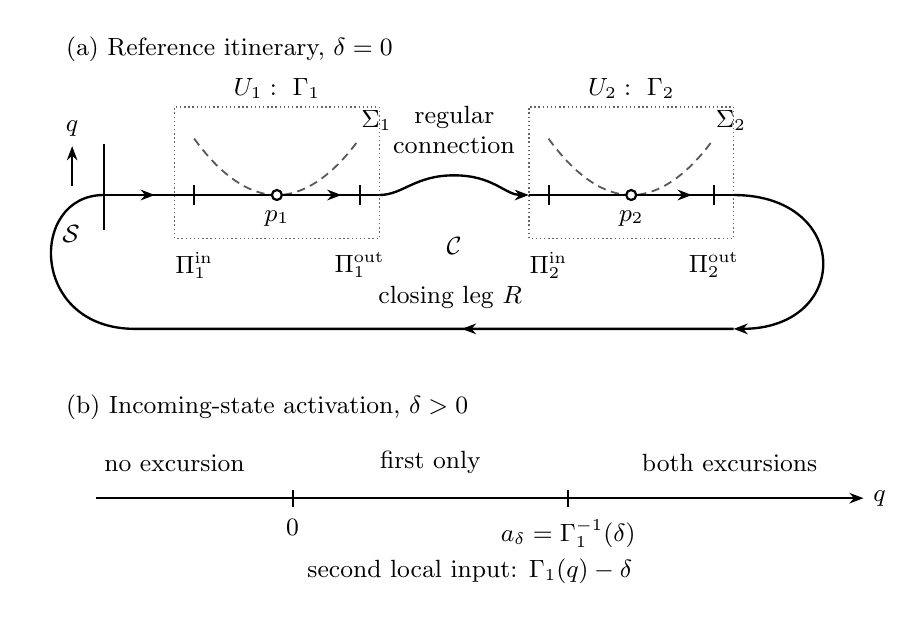
\begin{tikzpicture}[x=1cm,y=1cm,font=\small,
      orbit/.style={line width=.85pt},
      flow/.style={line width=.85pt,-{Stealth[length=1.8mm]}},
      seam/.style={line width=.65pt,densely dashed,black!65},
      box/.style={line width=.5pt,densely dotted,black!60},
      port/.style={line width=.75pt},
      axis/.style={line width=.55pt,-{Stealth[length=1.8mm]}}]
    \begin{scope}[yshift=2.9cm]
      \node[anchor=west] at (0,3.85)
        {(a) Reference itinerary, $\delta=0$};

      \draw[box] (1.5,1.45) rectangle (4.1,3.12);
      \draw[box] (6.0,1.45) rectangle (8.6,3.12);
      \node at (2.8,3.35) {$U_1:\ \Gamma_1$};
      \node at (7.3,3.35) {$U_2:\ \Gamma_2$};
      \draw[seam] (1.75,2.71625) parabola bend (2.8,2) (3.85,2.71625);
      \draw[seam] (6.25,2.71625) parabola bend (7.3,2) (8.35,2.71625);
      \node[anchor=west] at (3.75,2.95) {$\Sigma_1$};
      \node[anchor=west] at (8.25,2.95) {$\Sigma_2$};

      \draw[orbit] (.6,2) -- (4.1,2);
      \draw[flow] (4.1,2)
        .. controls (4.4,2) and (4.55,2.25) .. (5.05,2.25)
        .. controls (5.55,2.25) and (5.7,2) .. (6.0,2);
      \draw[orbit] (6.0,2) -- (8.6,2);
      \draw[flow] (8.6,2) .. controls (10.1,2) and (10.1,.3) .. (8.6,.3);
      \draw[orbit] (8.6,.3) -- (1.0,.3)
        .. controls (-.35,.3) and (-.35,2) .. (.6,2);
      \draw[flow] (.85,2) -- (1.25,2);
      \draw[flow] (3.2,2) -- (3.62,2);
      \draw[flow] (7.65,2) -- (8.07,2);
      \draw[flow] (6.0,.3) -- (5.15,.3);
      \node[align=center,text width=1.65cm] at (5.05,2.83)
        {regular\\connection};
      \node at (5.0,.7) {closing leg $R$};
      \node at (5.05,1.35) {$\mathcal C$};

      \draw[port] (.6,1.55) -- (.6,2.65);
      \draw[axis] (.2,2.12) -- (.2,2.62) node[above] {$q$};
      \node[anchor=east] at (.42,1.5) {$\mathcal S$};
      \draw[port] (1.75,1.87) -- (1.75,2.13);
      \draw[port] (3.85,1.87) -- (3.85,2.13);
      \draw[port] (6.25,1.87) -- (6.25,2.13);
      \draw[port] (8.35,1.87) -- (8.35,2.13);
      \node[below] at (1.75,1.4) {$\Pi_1^{\rm in}$};
      \node[below] at (3.85,1.4) {$\Pi_1^{\rm out}$};
      \node[below] at (6.25,1.4) {$\Pi_2^{\rm in}$};
      \node[below] at (8.35,1.4) {$\Pi_2^{\rm out}$};
      \draw[fill=white,line width=.8pt] (2.8,2) circle[radius=1.8pt];
      \draw[fill=white,line width=.8pt] (7.3,2) circle[radius=1.8pt];
      \node[below] at (2.8,1.93) {$p_1$};
      \node[below] at (7.3,1.93) {$p_2$};
    \end{scope}

    \node[anchor=west] at (0,2.2)
      {(b) Incoming-state activation, $\delta>0$};
    \draw[axis] (.5,1.05) -- (10.25,1.05) node[right] {$q$};
    \draw[port] (3.0,.94) -- (3.0,1.16);
    \draw[port] (6.5,.94) -- (6.5,1.16);
    \node[below] at (3.0,.9) {$0$};
    \node[below] at (6.5,.9) {$a_\delta=\Gamma_1^{-1}(\delta)$};
    \node at (1.5,1.5) {no excursion};
    \node at (4.75,1.5) {first only};
    \node at (8.55,1.5) {both excursions};
    \node at (5.25,.12) {second local input: $\Gamma_1(q)-\delta$};
  \end{tikzpicture}
  \caption{Schematic return geometry. Top: the reference itinerary at
    $\delta=0$, with dotted contact boxes $U_1,U_2$, dashed switching seams
    $\Sigma_1,\Sigma_2$, transverse ports and the return section
    $\mathcal S$. Arrows on the cycle show the direction of time; the
    section arrow orients $q$. Bottom:
    activation on the incoming state axis for $\delta>0$. The second
    passage is active when $\Gamma_1(q)-\delta>0$, so its threshold is
    $a_\delta$. For $\delta<0$, $a_\delta=\delta<0$ lies to the left of
    $0$, and only the second excursion occurs between them.}
  \label{fig:actual-return-geometry}
\end{figure}


\begin{lemma}[A common one-turn return tube]\label{lem:common-tube}
Let a compact embedded nonstationary reference cycle admit fixed tubular
coordinates $(\theta,w)$, with $\theta\in\R/\mathbb Z$, reference $w=0$
and section $\theta=0$. Suppose a finite smooth family of matched fields
has common local Lipschitz bounds on the tube and differs from the
reference field at $\lambda_0$ by $O(|\lambda-\lambda_0|)$. Fix contact cores and transverse ports with
strict margins, and strictly inactive connecting arcs. In every core,
assume that orbits with positive penetration enter the active region, stay
there and leave through the seam inside the core, and that the other orbits
touch the seam at most once.
If the angular clock remains positive and these local and port margins
persist, one can choose a common input interval and a parameter neighbourhood
on which the chronological composition is the first return map. It makes one
whole turn, with no further seam crossing or earlier section hit.
\end{lemma}

\begin{proof}
The matched form $X^-_\lambda+(h_\lambda)_+Z_\lambda$ has common
Lipschitz bounds. Compactness gives $\dot\theta\ge v_*>0$ on a smaller
tube; division by this clock and Gronwall comparison with $w=0$ give,
up to a first exit,
\[
 \begin{aligned}
 \left|\frac{dw}{d\theta}\right|&\le L|w|+K|\lambda-\lambda_0|,\\
 |w(\theta)|&\le e^L(|w(0)|+K|\lambda-\lambda_0|),\quad0\le\theta\le1.
 \end{aligned}
\]
Choose one input interval and parameter neighbourhood keeping this bound
strictly inside the tube, core and port margins. First-exit continuation
gives a full turn; the assumed core passages and inactive arcs exclude
further seam crossings, including for tangent inputs. The ports join on common
domains, and strict angular advance makes $\theta=1$ the next section hit.
The return image need not lie in the input interval.
\end{proof}

Lemma~\ref{lem:common-tube} gives a geometric criterion for the first-return
itinerary in item~2 of Definition~\ref{def:admissible-family}; Section~\ref{sec:sharpness} applies it
to the constructed families.

\begin{remark}[Cycles and fixed points]\label{rem:cycle-fixed-point}
After a common reduction, every periodic orbit sufficiently close to
$\mathcal C$ in the return tube meets the transverse section in $I$.
The first return is increasing and has no nontrivial finite-period orbit
whose iterates remain in the common local domain: if $P(q)>q$ or $P(q)<q$,
its successive iterates are strictly ordered. Thus these periodic orbits
correspond to fixed points in $I$, and isolation of the fixed point is
equivalent to isolation of the cycle in this tube.
\end{remark}

\subsection{Reversible passages and cancellation}
\label{sec:neutral-reference}\label{sec:center-multiplicity}

An active leaf pairs its two seam intersections by a decreasing
involution. We use it to identify the entry and exit of the passage.
The resulting relation between its first two coefficients determines
cancellation in the two-passage composition.

\begin{proposition}[Passage map near a quadratic grazing]
\label{prop:quadratic-passage}\label{prop:passage:quadratic}
For a local passage with the quadratic geometry~\eqref{eq:passage:local-geometry}
and fixed local transverse ports, there is a jointly smooth
signed companion $g(t,\lambda)$ on a two-sided interval such that
\begin{equation}\label{eq:passage:reversal}
 g(0,\lambda)=0,\qquad g_t(0,\lambda)=1,\qquad
 \iota g\iota=g^{-1},\qquad \iota(t)=-t.
\end{equation}
The passage in the inactive coordinate is
\begin{equation}\label{eq:passage:physical}
 \Gamma(q,\lambda)=q\quad(q\leq0),\qquad
 \Gamma(r^2,\lambda)=g(r,\lambda)^2\quad(r>0).
\end{equation}
Its first entry is $t=-r$ and its first moving exit is $g(r,\lambda)$.
On a common domain,
\begin{equation}\label{eq:passage:quadratic-jet}
 \Gamma(q,\lambda)
 =q+C_1(\lambda)q_+^{3/2}
       +\frac34C_1(\lambda)^2q_+^2
       +q_+^{5/2}L(\sqrt{q_+},\lambda),
\end{equation}
where $L$ is the restriction of a jointly smooth function, and
\begin{equation}\label{eq:passage:strength-jet}
 C_1(\lambda)=\frac43\mu(0,0,\lambda).
\end{equation}
The passage is an orientation-preserving $C^1$ local diffeomorphism, and the
companion, its inverse and the root profiles satisfy uniform bounds of every
prescribed order.
\end{proposition}

\begin{proof}
Divide the active field by its positive $t$ component. Let
$K(t,z,\lambda)$ be the $z$ coordinate where its orbit meets $t=0$.
Smooth finite-time ODE dependence gives $K(0,z,\lambda)=z$ and $K_z>0$
on a common smaller box. Since the active orbit equation has zero
$z$ component on the seam, $K_t(t,t^2,\lambda)=0$. Hence the seam
restriction $\widehat K(t,\lambda)=K(t,t^2,\lambda)$ satisfies
\[
 \begin{gathered}
 \widehat K_t=2tE(t,\lambda),\qquad
 E(t,\lambda)=K_z(t,t^2,\lambda)>0,\\
 \widehat K=t^2M(t,\lambda),\qquad
 M(t,\lambda)=2\int_0^1 sE(st,\lambda)\,ds.
 \end{gathered}
\]
Here $E(0,\lambda)=M(0,\lambda)=1$, so
$\mathcal N(t,\lambda)=t\sqrt{M(t,\lambda)}$ is a smooth increasing
local diffeomorphism. The active leaf pairs its seam intersections by
\[
 J=\mathcal N^{-1}\iota\mathcal N,\qquad
 J(0)=0,\quad J'(0)=-1,\quad J^2=\mathrm{id}.
\]

For input $q=r^2>0$, the inactive orbit first reaches the seam at $-r$.
Its active leaf has value $\widehat K(-r)>0$ and second intersection
$e=J(-r)>0$. The seam restriction decreases for $t<0$ and increases
for $t>0$; since $K_z>0$, the leaf $K=\widehat K(-r)$ lies strictly above the seam
precisely between $-r$ and $e$. The positive clock makes them the first
entry and first exit. In the normalized clock, $dh/dt=-2t$ on the seam, so the entry and exit
derivatives are exactly $2r$ and $-2e$. In the original physical time
they are multiplied by the positive clock factor. After exit the inactive orbit has $z=e^2$
and lies below the seam; port localization excludes further seam crossings.
Inputs $q<0$ stay below it and $q=0$ only touches it, giving the identity
passage on $q\le0$.

Set $g=J\iota$. Then $J^2=\iota^2=\mathrm{id}$ gives
$\iota g\iota=g^{-1}$ and $g'(0)=1$, while $e=g(r)$ proves
\eqref{eq:passage:physical}. For negative $t$, reversal gives
\begin{equation}\label{eq:passage:negative-companion}
 g(t,\lambda)=-\sqrt{\Gamma^{-1}(t^2,\lambda)}\qquad(t<0).
\end{equation}
This signed continuation records backward active travel; the forward
passage on negative $q$ is the identity.

Writing $g(t)=t+\rho t^2+\sigma t^3+O(t^4)$ and comparing cubic
coefficients in $(g\iota)^2=\mathrm{id}$ gives $\sigma=\rho^2$, the
classical jet relation for reversible maps~\cite{ofarrell2008,novaessilva2021}.
Taylor's integral remainder therefore gives
\[
 g(t)=t+\rho t^2+\rho^2t^3+t^4G(t,\lambda)
\]
with $G$ jointly smooth. Squaring at $t=\sqrt q>0$ gives
$C_1=2\rho$ and $C_2=3\rho^2=3C_1^2/4$, proving
\eqref{eq:passage:quadratic-jet}. Its parameter derivatives also give
joint $C^1$ regularity and $\Gamma_q\to1$ at zero.

For~\eqref{eq:passage:strength-jet}, note that $dz/dt=f(t,z)=h\mu/(1+h\alpha)$
and $K_t=-fK_z$. On the seam $f=0$ and $f_z=\mu$, so $E'(0)=-\mu(0,0)$.
Thus $\mathcal N(t)=t-\mu(0,0)t^2/3+O(t^3)$, and
$\mathcal N^{-1}\iota\mathcal N\iota$ has quadratic coefficient $2\mu(0,0)/3$;
squaring gives~\eqref{eq:passage:strength-jet}. Compactness, smooth dependence
on initial data and a common shrinking give uniform positivity and the
prescribed derivative bounds.
\end{proof}

Since $\partial_q=(2r)^{-1}\partial_r$, the $j$th state derivative of
$q^{5/2}L(\sqrt q,\lambda)$ is bounded by $C_jq^{5/2-j}$ on $q>0$, for every
fixed $j$ and after finitely many parameter derivatives. Its zero extension to
$q\le0$ is jointly $C^2$ in state and parameters.

Write $\Gamma_1,\Gamma_2$ for the two normalized passages.
The inactive connections preserve $q$, so chronological continuation gives
\begin{equation}\label{eq:passage:two-contact-map}
 \begin{aligned}
 Q_{m,\delta}(q,p)&=\delta+
 \Gamma_2\bigl(\Gamma_1(q,p,m,\delta)-\delta,p,m,\delta\bigr),\\
 P_{m,\delta}&=R_{p,m,\delta}\circ Q_{m,\delta},
 \end{aligned}
\end{equation}
where $R$ is the smooth orientation-preserving transition along the rest of
the cycle, the \emph{closing map}. Write $D=P-q$ and
$A_\nu(\lambda)=C_{1,\nu}(\lambda)$, the \emph{passage strengths}. When the
controls are independent we write $p=(a,b,\xi)$ and
$\lambda=(a,b,m,\delta,\xi)$, with $\xi$ in a fixed compact set. Throughout,
$m$ denotes the strength sum:
\begin{equation}\label{eq:net-strength}
 A_1(p,m,\delta)+A_2(p,m,\delta)=m,\qquad A(p)=A_1(p,0,0).
\end{equation}
The individual strengths and all higher profiles may depend on every
parameter. After reduction, $A$ has fixed sign with
$|A(p)|\ge A_*>0$, and the two passage strengths have opposite signs. The jets of the closing map are
\begin{equation}\label{eq:regular-jets}
 a=R(0),\qquad b=R'(0)-1,\qquad c=\tfrac12R''(0).
\end{equation}
In particular, the aligned multiplier is $k(p)=R'_{p,0,0}(0)=1+b>0$.
Taylor division gives
\begin{equation}\label{eq:quartic-closing-division}
 R(y)=a+(1+b)y+c(\lambda)y^2+y^3S(y,\lambda).
\end{equation}
At the reference $a=b=m=\delta=0$. The aligned curvature
$c_0(p)=\tfrac12R''_{p,0,0}(0)$ has fixed nonzero sign and a uniform
strict margin; after shrinking, $R''$ retains that sign at every relevant
input. Its value may vary with the parameters. The attainment results use
the condition
\begin{equation}\label{eq:rank}
 \operatorname{rank}D_\lambda(a,b,m,\delta)=4
 \quad\hbox{at the reference field},
\end{equation}
which makes $(a,b,m,\delta,\xi)$ local parameter coordinates.

\begin{lemma}[Cancellation at aligned thresholds]
\label{lem:passage:finite-inverse}
On $\delta=0$, the composition has the root-profile form
\begin{equation}\label{eq:passage:aligned-jet}
 Q_{m,0}(q)=q+mq_+^{3/2}+\frac34m^2q_+^2
                  +q_+^{5/2}L_0(\sqrt{q_+},a,b,m,\xi).
\end{equation}
Consequently, on the whole slice $m=\delta=0$,
\begin{equation}\label{eq:passage:finite-cancellation}
 Q_{0,0}(q)=q+q_+^{5/2}L_0(\sqrt{q_+},a,b,0,\xi)
\end{equation}
is jointly $C^2$. Only the leading strengths have to cancel.
\end{lemma}

\begin{proof}
On a common smaller domain positive inputs and intermediate images stay
positive. The cubic companion jets and $A_1+A_2=m$ give
\[
 g_2g_1(t)=t+\frac m2t^2+\frac{m^2}{4}t^3
                      +t^4G_0(t,a,b,m,\xi),
\]
with $G_0$ jointly smooth. Squaring proves
\eqref{eq:passage:aligned-jet}; for $q\le0$ both passages are identity.
At $m=0$ the remaining $q_+^{5/2}$ profile has the joint $C^2$
extension proved above.
\end{proof}

The grazing thresholds on the incoming section are
\begin{equation}\label{eq:passage:true-thresholds}
 0\quad\hbox{and}\quad a_\delta=\Gamma_1^{-1}(\delta,\lambda).
\end{equation}
Here $a_\delta$ labels the second threshold; it does not denote a
parameter derivative. The second local input is
$I_2=\Gamma_1(q,\lambda)-\delta$.
The increasing first passage has derivative near one, so its inverse
exists on a common interval and
\begin{equation}\label{eq:passage:threshold-formula}
 a_\delta=\delta\quad(\delta\le0),\qquad
 a_\delta=\bigl[g_1^{-1}(\sqrt\delta,\lambda)\bigr]^2
                                                \quad(\delta>0).
\end{equation}
Thus $a_\delta$ has the sign of $\delta$, $|a_\delta|\le2|\delta|$,
and for positive separation
$a_\delta=\delta-C_{1,1}(\lambda)\delta^{3/2}+O(\delta^2)$ with a
smooth positive-root profile. It is jointly $C^1$; as a function of the
independent separation variable $\delta$, it is not $C^2$ at $\delta=0$
when $C_{1,1}\ne0$.
For $\delta>0$, the intervals $q<0$, $0<q<a_\delta$, $q>a_\delta$
have respectively no excursion, only the first, and both excursions.
For $\delta<0$, the corresponding intervals are $q<\delta$,
$\delta<q<0$, $q>0$, with only the second excursion in the middle.
At either endpoint its excursion becomes a tangency touch. At alignment,
negative inputs are inactive, zero touches both contacts and positive
inputs make both excursions.

On the aligned cancelling slice, the closing expansion gives
\begin{equation}\label{eq:center-displacement}
 D_{0,0}(q,p)=a+bq+c_0(p)q^2
       +q_+^{5/2}M(\sqrt{q_+},p)+q^3S(q,p),
 \qquad c_0(p)=\tfrac12R_{p,0,0}''(0)\ne0.
\end{equation}
The root remainder is jointly $C^2$, with bounds
$|\partial_q^j\partial_p^\beta(q^{5/2}M)|\le C_{j,\beta}q^{5/2-j}$
for $j\le2$. At $a=b=0$ the reference displacement consequently has
$D(0)=D_q(0)=0$ and $D_{qq}(0)=2c_0\ne0$.
The return map is jointly $C^1$ in state and parameters. Since both strengths
are nonzero, $P_\lambda$ is $C^2$ at both thresholds if and only if
$m(\lambda)=\delta(\lambda)=0$; otherwise a nonzero coefficient of order
$q^{3/2}$ survives at one of the thresholds. For the counting bounds, fixed points at thresholds are counted as distinct
zeros; no smooth multiplicity is used at a non-$C^2$ threshold.

A smooth increasing change of transverse coordinate $x=\phi(q)$, $\phi(0)=0$,
$\phi'(0)=s>0$, changes the reference coefficients to $\widetilde c_0=c_0/s$
and $\widetilde A_\nu=A_\nu(\lambda_0)/\sqrt{s}$; the terms involving $\phi''(0)$
cancel at a fixed point with unit multiplier. In particular $c_0/A_1(\lambda_0)^2$
does not depend on the coordinate. The odd root lift $t\sqrt{\phi(t^2)/t^2}$
preserves reversal, and nonlinear terms of $\phi$ first affect the order
$5/2$, so the coefficient law of Proposition~\ref{prop:quadratic-passage} is
preserved. These invariants let us check the sign conditions in any such
section coordinate and compare the constants in the weighted limits.

\subsection{Regular connections and auxiliary parameters}

We now show how regular connecting maps lead to this form, and how families
with dependent controls are handled.

\begin{proposition}[Return map through regular connections]
\label{prop:field-recognition}\label{prop:passage:field-recognition}
In the common geometry above, let $S_1,S_2$ be the regular transitions in
positive penetration coordinates, with all intermediate images in their
common domains. They are smooth and increasing, with common positive
derivative margins. If the second local level is $\delta_2$, then
\begin{equation}\label{eq:passage:unreduced-return}
 P=S_2\circ\Pi_2\circ S_1\circ\Gamma_1,
 \qquad\Pi_2(z)=\delta_2+\Gamma_{2,\mathrm{loc}}(z-\delta_2)
\end{equation}
has the transported form
\begin{equation}\label{eq:passage:recognized-return}
 P(q)=R\{\delta+\Gamma_2(\Gamma_1(q)-\delta)\},
 \qquad\delta=S_1^{-1}(\delta_2),\quad R=S_2\circ S_1.
\end{equation}
The second passage retains reversal and the coefficient law. The four
controls are smooth functions of $\lambda$, and under~\eqref{eq:rank} they
give a chart $(a,b,m,\delta,\xi)$ with $m=C_{1,1}+C_{1,2}$.
\end{proposition}

\begin{proof}
The first transition is increasing by admissibility. The inactive reference
monodromy preserves transverse orientation, so $S_2'>0$ at the reference as
well; smooth dependence gives common positive derivative margins after
reduction.
Set $T(x)=S_1(\delta+x)-\delta_2$ and
$\Gamma_2=T^{-1}\Gamma_{2,\mathrm{loc}}T$.
Then $T(0)=0$, $T'>0$, and
$S_1^{-1}\Pi_2S_1(y)=\delta+\Gamma_2(y-\delta)$, proving the formula.
The signed root lift is
\[
 H(t)=t\sqrt{T(t^2)/t^2},\qquad
 T(t^2)/t^2=\int_0^1T'(st^2)\,ds,\qquad
 g_2=H^{-1}g_{2,\mathrm{loc}}H.
\]
The quotient is smooth, positive and even. Thus $H$ is odd, increasing,
with a smooth bounded inverse on a common root interval; conjugation
preserves reversal. Squaring for $t>0$ gives the transported passage.
For $\ell=T'(0)$ its first coefficients are
$C_{1,2}=\sqrt\ell\,C_{1,2,\mathrm{loc}}$ and
$C_{2,2}=\ell C_{2,2,\mathrm{loc}}$, so $C_{2,2}=3C_{1,2}^2/4$.
Nonlinear terms in $T$ first enter the order-$5/2$ remainder.
The transported first integral is $S_1^{-1}$ of the old one; its level,
first entry and moving first exit follow the same trajectories.
The common itinerary therefore gives the chronological first return.
Smooth parameter dependence gives the four control functions, and
under~\eqref{eq:rank} the submersion theorem gives the asserted chart.
\end{proof}

Within an admissible family, finite-time dependence and the implicit
function theorem for hitting times give smooth regular transitions with
common clock, derivative and domain margins. The opposite strength signs
and nonzero closing curvature persist in a neighbourhood; cancellation is
imposed only at the reference.

For dependent controls we introduce independent auxiliary parameters for
the estimates.

\begin{lemma}[Independent auxiliary strength and separation]
\label{lem:auxiliary-controls}
Let a jointly smooth finite-parameter family have the normalized return
\[
 \begin{gathered}
 P_\lambda(q)=R_\lambda\bigl(\widehat\delta(\lambda)+
 \Gamma_{2,\lambda}(\Gamma_{1,\lambda}(q)
                              -\widehat\delta(\lambda))\bigr),\\
 \widehat m(\lambda)=C_{1,1}(\lambda)+C_{1,2}(\lambda),
 \end{gathered}
\]
with the signed companions of Proposition~\ref{prop:quadratic-passage}.
Near a reference with $\widehat m=\widehat\delta=0$, there is a jointly
smooth root-profile family with independent auxiliary parameters
$(m,\delta)$, the same coefficient law and the identity
$C_{1,1}+\widetilde C_{1,2}=m$ for all auxiliary $(m,\delta)$,
whose return satisfies
\[
 \widetilde P_{\lambda,\widehat m(\lambda),
                       \widehat\delta(\lambda)}=P_\lambda.
\]
The closing map remains $R_\lambda$, and all profiles satisfy uniform
bounds.
\end{lemma}

\begin{proof}
Put $\iota(t)=-t$, $J_2=g_{2,\lambda}\iota$ and
$\mathcal N_2(t,\lambda)=(t-J_2(t,\lambda))/2$.
Since $J_2^2=\id$, $\mathcal N_2J_2=\iota\mathcal N_2$ and
$\mathcal N_2'(0)=1$, so $\mathcal N_2$ is a jointly smooth increasing
local normalizer. For $s=m-\widehat m(\lambda)$ set
\[
 \mathcal N_s(t,\lambda)=\mathcal N_2(t,\lambda)-\frac s4t^2,
 \qquad \widetilde g_2=\mathcal N_s^{-1}\iota\mathcal N_s\iota.
\]
A common shrinking keeps $\mathcal N_s'>0$, and the parameter inverse
function theorem gives its joint smooth inverse. Thus $\widetilde g_2$
is tangent to the identity, satisfies
$\iota\widetilde g_2\iota=\widetilde g_2^{-1}$, and equals $g_{2,\lambda}$
when $s=0$. If $\mathcal N_2=t+d_2t^2+O(t^3)$, the quadratic coefficient
of $\mathcal N_2^{-1}\iota\mathcal N_2\iota$ is $-2d_2$.
The change therefore raises the quadratic coefficient of $\widetilde g_2$
by $s/2$.
Define $\widetilde\Gamma_2(x)=x$ for $x\le0$ and
$\widetilde\Gamma_2(t^2)=\widetilde g_2(t)^2$ for $t>0$.
Its second-passage strength is $\widetilde C_{1,2}=C_{1,2}+s$, so
$C_{1,1}+\widetilde C_{1,2}=\widehat m+s=m$.
Reversibility gives its coefficient law and smooth root remainder.
Replace the second passage in the return by $\widetilde\Gamma_2$ and
use the independent translation $\delta$. This recovers the original
return at $(m,\delta)=(\widehat m(\lambda),\widehat\delta(\lambda))$. Joint
smoothness on compact reductions gives the uniform bounds.
\end{proof}

For the estimates below, a family with dependent controls is first treated
in this auxiliary root-profile family and then restricted to
$(m,\delta)=(\widehat m(\lambda),\widehat\delta(\lambda))$.
This convention concerns estimates of return maps; it asserts no field
realization of the auxiliary profiles.

\subsection{Divisions and estimates up to the thresholds}

Where both passages are active, the return admits a division in root
profiles. To cover the thresholds as well, we also estimate the difference
from the aligned return in the coordinate $q$.

\begin{lemma}[Division and estimates up to the thresholds]
\label{lem:exact-value-division}
There are common $r_0>0$, $v_0=1/4$ and a small parameter neighbourhood
in $(m,p)$
such that, for $0<r\le r_0$, $|v|\le v_0$, $q=r^2$ and $\delta=r^2v$,
both passages are active and the return has the expression
\begin{equation}\label{eq:actual-both-active-division}
 Q-q=mr^3+\tfrac34m^2r^4+r^5L_0+\delta rH,
 \qquad H(0,0,0,p)=\tfrac32A(p),
\end{equation}
where $L_0,H$ are restrictions of jointly smooth functions of $(r,m,v,p)$
on the signed box $|r|\le r_0$, $|v|\le v_0$, with the same parameter
neighbourhood. For arbitrary relative sizes and either sign of
$q$ and $\delta$ in the common local domain, including the thresholds,
\begin{equation}\label{eq:quartic-global-value}
 |Q-q-mq_+^{3/2}|
 \le K\{m^2q_+^2+q_+^{5/2}
       +|\delta|\sqrt{q_++|\delta|}+|\delta|q_+^{3/2}\}
\end{equation}
with a common constant.
\end{lemma}

\begin{proof}
Write $g_\nu(t,\lambda)=tT_\nu(t,\lambda)$ with $T_\nu$ jointly smooth
and $T_\nu(0,\lambda)=1$. For signed $r$ and $\delta=r^2v$, put
\[
 U=T_1(r,\lambda)^2,\quad W=U-v,\quad s_2=r\sqrt W,
 \qquad K_0=v+WT_2(s_2,\lambda)^2.
\]
Since $T_1(0,\lambda)=1$, one common reduction gives $T_1^2>3/4$.
For $|v|\le v_0=1/4$ this implies $W=T_1^2-v>1/2$. These expressions are smooth and
$Q(r^2)=r^2K_0$ exactly for $r>0$. Since $K_0(0,m,v,p)=1$,
joint Hadamard division gives $K_0-1=r\mathcal Q$. Aligned cancellation gives
$\mathcal Q(r,m,0,p)=m+\tfrac34m^2r+r^2L_0(r,m,p)$; division in the independent
variable $v$ then gives the exact identity
\begin{equation}\label{eq:quartic-Hadamard}
 \mathcal Q=m+\tfrac34m^2r+r^2L_0+vH(r,m,v,p),
 \qquad H(0,0,0,p)=\tfrac32A(p).
\end{equation}
Indeed, the first root jet at $r=0$ is
$A_1+A_2(1-v)^{3/2}$, whose $v$ derivative at cancellation is
$-3A_2/2=3A(p)/2$. The profile arguments contain $\delta=r^2v$.
Multiplication by $r^3$ proves
\eqref{eq:actual-both-active-division}.

Under~\eqref{eq:rank}, hold $(a,b,m,\xi)$ fixed. For dependent controls,
write $p$ for the original physical parameters and hold $(p,m)$ fixed in
the auxiliary family of Lemma~\ref{lem:auxiliary-controls}, varying only
its auxiliary separation $\delta$. After integration, restrict to the
observed controls as agreed above. Put $y=\Gamma_1(q)-\delta$. The total
derivative is
\begin{equation}\label{eq:quartic-total-detuning}
 Q_\delta=1-\Gamma_{2,q}(y)
 +\Gamma_{2,q}(y)\Gamma_{1,\delta}(q)+\Gamma_{2,\delta}(y).
\end{equation}
The profile parameter derivatives are $O(x_+^{3/2})$. Integrate \eqref{eq:quartic-total-detuning} from zero to $\delta$,
with the indicated quantities held fixed. At an intermediate separation $t$,
$y_+=(\Gamma_1(q,t)-t)_+\le Kq_++|t|$. Joint $C^1$ regularity
and the smooth profiles give, including at active arguments equal to zero,
\[
 |\Gamma_{\nu,q}(x)-1|\le K\sqrt{x_+},\qquad
 |\Gamma_{\nu,t}(x)|\le Kx_+^{3/2}.
\]
Thus $|Q_t|\le K[\sqrt{q_++|t|}+q_+^{3/2}]$, and
\begin{equation}\label{eq:quartic-global-detuning}
 |Q_{m,\delta}-Q_{m,0}|
 \le K|\delta|[\sqrt{q_++|\delta|}+q_+^{3/2}].
\end{equation}
Together with \eqref{eq:passage:aligned-jet} this proves
\eqref{eq:quartic-global-value}.
\end{proof}

\begin{remark}[Checking the hypotheses]\label{cor:field-criterion}
With the prescribed contact geometry, transverse coorientation and
common first-return itinerary, the remaining conditions involve finitely
many jets. The transported strengths are $A_\nu=\tfrac43\mu_\nu(0,0)$;
transport from an initial second-port coordinate multiplies its strength by
$\sqrt{S_1'(\delta)}$, as in Proposition~\ref{prop:field-recognition}.
At the reference, check $A_1=-A_2\ne0$, $R(0)=0$, $R'(0)=1$ and
$c_0=R''(0)/2\ne0$. These conditions give admissibility and the upper
bounds of Theorem~\ref{thm:six-main} and part~1 of
Theorem~\ref{thm:main-saturation-summary}. Attainment additionally uses
\eqref{eq:rank}; the saturation and fourfold-cycle conclusions use the
sign sector specified in Theorems~\ref{thm:main-saturation-summary}
and~\ref{thm:actual-quartic-summary}.
\end{remark}

The curvature of this composition gives the count in the next section, and
the value estimates locate the six-cycle configurations.

\section{Sharp cyclicity}
\label{sec:curvature-graph}

We count fixed points by following the zeros of $P''$, which we call the
curvature of the return. Where both passages are active and the state is
large compared with the separation (the outer region), these zeros lie on a
separation graph with at most one positive critical point; estimates near the
thresholds (the threshold layer) fix the sign of $P''$ there. Together they
give the upper bounds on the whole interval $I$. We then construct
configurations attaining the bounds under~\eqref{eq:rank}.

An active three-halves term has curvature proportional to \(q^{-1/2}\).
In the outer region, where both passages are active, \(q=r^2\) and \(J=rP''\) remove
this singular factor, while \(v=\delta/q\) measures separation relative
to the state. With the aligned multiplier \(k(p)=1+b>0\), their first-order balance is
\[
 J=2c_0r+\frac{3k}{4}m-\frac{3kA}{8}v
       +O\bigl((r+|m|+|v|)^2\bigr).
\]
The strength $A\ne0$ makes the curvature equation transverse in $v$.
Exact division then gives a separation graph $\Delta$ with
$\Delta_r=r\mathcal W$; the closing curvature $c_0\ne0$ makes
$\mathcal W$ strictly monotone. These two reductions give at most one
positive critical point.

\subsection{The exact curvature-zero graph}

Let \(g_\nu\) be the signed-root companion in
Proposition~\ref{prop:quadratic-passage}. Its dependence on
\((p,m,\delta)\) is suppressed in the notation. Define smooth functions
\begin{equation}\label{eq:root-profiles}
 T_\nu(u)=g_\nu(u)/u,\quad
 \ell_\nu(u)=T_\nu(u)^2+\tfrac{u}{2}(T_\nu^2)'(u),
 \quad H_\nu(u)=\tfrac12\ell_\nu'(u).
\end{equation}
The quotient is filled in smoothly at \(u=0\), with \(T_\nu(0)=1\).
For \(u>0\),
\begin{equation}\label{eq:passage-derivatives}
 \Gamma_\nu'(u^2)=\ell_\nu(u),\qquad
 \Gamma_\nu''(u^2)=u^{-1}H_\nu(u),\qquad
 \ell_\nu(0)=1,\quad H_\nu(0)=\tfrac34 A_\nu.
\end{equation}
These are exact identities obtained by differentiating
\(\Gamma_\nu(u^2)=g_\nu(u)^2\).

For \(r>0\), put
\begin{equation}\label{eq:J-definition}
 q=r^2,\quad \delta=r^2v,\quad
 J(r,m,v,p)=rP_{m,r^2v}''(r^2,p).
\end{equation}
Choose a fixed small \(0<\eta\le v_0=1/4\), within the box of Lemma~\ref{lem:exact-value-division}. All profiles in the following
calculation are evaluated at \(\delta=r^2v\).
Write
\[
 U=T_1(r)^2,\qquad W=U-v,\qquad s_2=r\sqrt{W}.
\]
After a fixed common shrinking, \(W>1/2\) for \(|v|\le\eta\).
The two excursions are then both active and the exact downstream
penetration is \(y=r^2W>0\). Chain differentiation gives
\begin{align}
 Q&=r^2\{v+WT_2(s_2)^2\},&
 Q'&=\ell_2(s_2)\ell_1(r),\label{eq:Q-outer}\\
 Q''&=r^{-1}\{\ell_2(s_2)H_1(r)
       +W^{-1/2}H_2(s_2)\ell_1(r)^2\}.\label{eq:Q-curvature}
\end{align}
Consequently
\begin{align}\label{eq:J-exact}
 J={}&rR''(Q)[\ell_2(s_2)\ell_1(r)]^2\\
 &+R'(Q)\{\ell_2(s_2)H_1(r)
               +W^{-1/2}H_2(s_2)\ell_1(r)^2\}.\notag
\end{align}
Every expression on the right is a root profile, jointly smooth through
\(r=0\).

\begin{lemma}[Root curvature and its zero graph]\label{lem:curvature-profile}
The function \(J\) has a joint smooth extension on a common box
in \((r,m,v,p)\). At its root boundary,
\begin{equation}\label{eq:J-boundary}
 J(0,m,v,p)
 =\tfrac34 R'_{p,m,0}(0)
     \{A_1(p,m,0)+A_2(p,m,0)(1-v)^{-1/2}\}.
\end{equation}
In particular,
\begin{equation}\label{eq:J-transverse}
 J_v(0,0,0,p)=-\tfrac38 R'_{p,0,0}(0)A(p)\ne0.
\end{equation}
There is exactly one smooth graph \(v=V(r,m,p)\), with
\(|V|<\eta\), on which \(J=0\) in this box.
\end{lemma}

\begin{proof}
Formula~\eqref{eq:J-exact} proves smoothness, and
\eqref{eq:passage-derivatives} at \(r=s_2=0\) gives
\eqref{eq:J-boundary}. Differentiation in \(v\) gives
\eqref{eq:J-transverse}. First choose \(\eta\) so that \(J_v\) has
the strict sign \(-A\) and a uniform nonzero margin on the root
boundary. The signs of \(J(0,0,-\eta,p)\) and
\(J(0,0,\eta,p)\) are opposite. Compactness in the remaining
parameters permits one further shrinking of \(r,m\) on which these
properties persist throughout the box. The implicit function theorem,
existence by the endpoint signs, and strict monotonicity in \(v\)
give the asserted unique graph.
\end{proof}

The boundary value of the graph is exact:
\begin{equation}\label{eq:V-boundary}
 V(0,m,p)=1-\left(\frac{-A_2(p,m,0)}{A_1(p,m,0)}\right)^2,
 \qquad V_m(0,0,p)=\frac{2}{A(p)}.
\end{equation}
Indeed the ratio equals \(1-m/A_1(p,m,0)\); both individual strengths
retain their dependence on \(m\).

To bound the positive critical points of the separation graph
\(r\mapsto r^2V(r,m,p)\) on a fixed interval, divide first along
the cancelling slice and then in the independent strength variable.
Finite cancellation gives
\begin{equation}\label{eq:Q-aligned}
 Q_{0,0}(q,p)=q+q_+^{5/2}L(\sqrt{q_+},p).
\end{equation}
For positive \(q=r^2\) it follows, by differentiation in \(q\),
that
\begin{equation}\label{eq:center-curvature}
 P_{0,0}''(r^2,p)=2c_0(p)+rN(r,p),\qquad
 c_0(p)=\tfrac12R_{p,0,0}''(0),
\end{equation}
where \(N\) is jointly smooth. The offset and linear jets are allowed
to vary in \(p\) throughout this identity.

Let \(V_0(r,p)=V(r,0,p)\). Since \(J(r,0,V_0,p)=0\), the mean-value
identity in the independent variable \(v\) yields
\[
 0=r\{2c_0+rN\}
       +V_0\int_0^1J_v(r,0,tV_0,p)\,dt.
\]
The integral has a nonzero common margin. Therefore \(V_0=rB_\Delta(r,p)\)
with \(B_\Delta\) smooth and
\begin{equation}\label{eq:B-boundary}
 B_\Delta(0,p)=\frac{16c_0(p)}{3R'_{p,0,0}(0)A(p)}.
\end{equation}
Hadamard division in \(m\) now gives the exact identity
\begin{equation}\label{eq:V-division}
 V(r,m,p)=mH_\Delta(r,m,p)+rB_\Delta(r,p),\qquad
 H_\Delta(0,0,p)=\frac{2}{A(p)}.
\end{equation}

Define the separation graph
\begin{equation}\label{eq:Delta-definition}
 \Delta(r,m,p)=r^2V(r,m,p).
\end{equation}
Its derivative factors exactly:
\begin{equation}\label{eq:Delta-derivative}
 \Delta_r=r\mathcal W,\qquad \mathcal W=2V+rV_r.
\end{equation}
The boundary coefficients in \eqref{eq:V-division} give
\begin{equation}\label{eq:W-boundary}
 \mathcal W_m(0,0,p)=\frac4{A(p)},\qquad
 \mathcal W_r(0,0,p)=3B_\Delta(0,p)
   =\frac{16c_0(p)}{R'_{p,0,0}(0)A(p)}\ne0.
\end{equation}
Joint smoothness and compactness in \(p\) give a common smaller box
on which \(\mathcal W_r\) has a uniform nonzero margin with sign
\(c_0/A\).

\begin{proposition}[At most one critical point of the separation graph]\label{prop:one-fold-graph}
For fixed \((m,p)\), the graph \(r\mapsto\Delta(r,m,p)\) has at most
one positive critical point on a common interval. Any such point
is nondegenerate. In the outer region \(|\delta|/r^2\le\eta\),
\begin{equation}\label{eq:curvature-factor}
 P_{m,\delta}''(r^2,p)
 =r^{-3}\mathcal U(r,m,\delta/r^2,p)
                  [\delta-\Delta(r,m,p)],
\end{equation}
where \(\mathcal U\) is jointly smooth and nonzero, of sign \(-A\).
For fixed parameters the zeros of \(P''\) in the outer region have total
multiplicity at most two.
\end{proposition}

\begin{proof}
For fixed \((m,p)\), \(\mathcal W\) is strictly monotone and has
at most one positive zero. At that zero,
\(\Delta_{rr}=r\mathcal W_r\ne0\). Hence \(\Delta\) has at most
two monotone branches.

For the factorization, define
\[
 \mathcal U(r,m,v,p)
  =\int_0^1J_v(r,m,V+t(v-V),p)\,dt .
\]
The derivative bound from Lemma~\ref{lem:curvature-profile}
gives its sign and nonvanishing. The exact mean-value identity is
\(J=(v-V)\mathcal U\). Substituting
\(v=\delta/r^2\) in \eqref{eq:J-definition} gives
\eqref{eq:curvature-factor}.
A horizontal line meets this graph in at most two transverse
points, or at its sole positive critical point. Transverse intersections are simple;
an intersection at the nondegenerate critical point has order two.
Changing from \(r>0\) to \(q=r^2\) is a smooth local diffeomorphism,
and the prefactor in \eqref{eq:curvature-factor} never vanishes.
This proves the multiplicity assertion as well as the distinct count.
\end{proof}

We now treat the complement of the outer region, where an active input may
be arbitrarily close to its threshold.

\subsection{The count on the whole interval}\label{sec:inner}

Use the thresholds $0$ and $a_\delta=\Gamma_1^{-1}(\delta)$
from \eqref{eq:passage:true-thresholds}, with the active intervals determined
there. All constants are uniform on the fixed parameter reduction.

Where both passages are active in the threshold layer, compare the difference of the singular
curvatures with their sum. Separation keeps the active inputs at a fixed
relative distance; the difference then dominates both the relative error
and the bounded closing curvature.

Put \(\vartheta=|\delta|\), \(\sigma=\sgn\delta\), and let \(L\ge2\) be fixed.
The strengths satisfy, uniformly,
\[
 A_1(p,m,\delta)=A(p)+O(|m|+\vartheta),\qquad
 A_2(p,m,\delta)=-A(p)+O(|m|+\vartheta).
\]
The smooth root profiles in \eqref{eq:passage:quadratic-jet} yield
\begin{align}
 \Gamma_\nu'(x)
  &=1+\tfrac32 A_\nu\sqrt{x}+O(x),\label{eq:inner-derivative}\\
 \Gamma_\nu''(x)
  &=\tfrac34 A_\nu x^{-1/2}+O(1),\qquad x>0.\label{eq:inner-curvature}
\end{align}
Differentiating the smooth root profiles gives these remainders and their
required derivative bounds. Each $\Gamma_\nu'$ is uniformly positive and
bounded, with active curvature of the sign of its strength.

For \(0<q\le L\vartheta\),
\begin{equation}\label{eq:first-correction}
 |\Gamma_1(q)-q|\le Kq^{3/2}\le K L^{3/2}\vartheta^{3/2}.
\end{equation}
After reducing \(\vartheta\), this is at most \(\vartheta/2\).
The inverse derivative estimates give \(\vartheta/2<a_\vartheta<2\vartheta\).
Every positive penetration in this layer is at most \((L+2)\vartheta\).

\begin{lemma}[Curvature signs in the threshold layer]\label{lem:event-layer}
For every fixed \(L\ge2\), one may choose common sufficiently small
bounds on \(|m|\) and \(\vartheta=|\delta|\) such that, for \(0<|\delta|\),
the signs of \(P''\) are
\begin{equation}\label{eq:event-signs}
 \sgn P''=
 \begin{cases}
 \sgn c,&q<\min(0,a_\delta),\\
 \sgn(\delta A),&\min(0,a_\delta)<q<\max(0,a_\delta),\\
 \sgn(-\delta A),&
       q>\max(0,a_\delta),\quad q\le L|\delta|.
 \end{cases}
\end{equation}
Both passages are active on the last interval. There is no zero of \(P''\) in any
of these open regions. In the active regions
\(|Q''|\ge\kappa_L \vartheta^{-1/2}\) for a uniform \(\kappa_L>0\).
The estimates are uniform up to the thresholds.
\end{lemma}

\begin{proof}
Below both thresholds both passages are inactive, so \(Q=q\) and
\(P''=R''\), with sign \(c\).

If \(\delta=\vartheta>0\), the one-active interval is \(0<q<a_\vartheta\), where
\(Q=\Gamma_1(q)\). Its curvature has sign \(A\), and
\eqref{eq:inner-curvature} gives
\(|Q''|\ge\kappa_L(2\vartheta)^{-1/2}\) after shrinking.
If \(\delta=-\vartheta<0\), that interval is \(-\vartheta<q<0\), where
\(Q=-\vartheta+\Gamma_2(q+\vartheta)\). Its curvature has sign \(-A\) and the same
uniform lower bound.

Where both passages are active, put
\[
 y=\Gamma_1(q)-\delta>0.
\]
The exact chain rule is
\[
 Q''=\Gamma_2'(y)\Gamma_1''(q)
          +\Gamma_2''(y)\Gamma_1'(q)^2.
\]
Equations~\eqref{eq:inner-derivative}--\eqref{eq:first-correction}
therefore give
\begin{equation}\label{eq:relative-inner-error}
 Q''=\tfrac34 A(q^{-1/2}-y^{-1/2})+E,\qquad
 |E|\le C_L(\sqrt \vartheta+\vartheta+|m|)
                 (q^{-1/2}+y^{-1/2}).
\end{equation}
Each error is measured relative to the sum of the two singular
weights, so the formula remains uniform as either positive argument tends
to zero.

By \eqref{eq:first-correction},
\(\sigma(q-y)\ge \vartheta/2\) and \(q,y\le(L+2)\vartheta\). Hence
\[
 -\sigma\frac{q^{-1/2}-y^{-1/2}}{q^{-1/2}+y^{-1/2}}
 =\frac{|q-y|}{(\sqrt q+\sqrt y)^2}
 \ge\frac1{8(L+2)}=:d_L>0.
\]
First reduce \(|m|\), and then \(\vartheta\), so the error in
\eqref{eq:relative-inner-error} is less than half the principal bound.
Thus \(\sgn Q''=\sgn(-\sigma A)\) and
\(|Q''|\ge\kappa_L\vartheta^{-1/2}\), throughout the open two-active layer.

Finally the exact closing-leg chain rule is
\[
 P''=R''(Q)(Q')^2+R'(Q)Q''.
\]
The first term is uniformly bounded, whereas \(R'\) has a positive
margin and the preceding active curvature bound diverges as
\(\vartheta\downarrow0\). A further fixed reduction proves
\eqref{eq:event-signs}.
\end{proof}

\begin{proposition}[Upper bound on the whole interval]\label{prop:common-count}
On a sufficiently small interval $I=(-q_0,q_0)$, common to the family, every
return map $P_\lambda$, $\lambda\in U$, has at most six fixed points.
\end{proposition}

\begin{proof}
First choose the outer box and its fixed \(\eta\) in
Lemma~\ref{lem:curvature-profile}. Set \(L=1/\eta\ge2\), shrinking
\(\eta\) if needed. Apply Lemma~\ref{lem:event-layer} with this one
\(L\): reduce the common strength bound and then the separation bound.
All further reductions are made inside the first-return domain of
Definition~\ref{def:admissible-family}. Choose \(q_0,\delta_0\) so both thresholds remain
strictly inside \(I=(-q_0,q_0)\), for example using
\(\delta_0<q_0/4\) and the uniform inverse derivative bound.

For \(\delta\ne0\), \(P''\) has no zeros in the three regions
of~\eqref{eq:event-signs}. Any remaining zero of \(P''\) has
\(q>L|\delta|>0\), so it lies in the outer region \(|\delta|/q<\eta\).
Proposition~\ref{prop:one-fold-graph} exhausts this region and gives at most
two zeros of \(P''\). At each threshold \(P''\) has a singularity with
nonzero coefficient, so a threshold is not a zero of \(P''\).

The derivative \(P'\) is continuous at the thresholds.
It is strictly monotone on at most five consecutive pieces: the two
thresholds and at most two zeros of \(P''\) are the only possible
divisions. If the signs of \(P''\) on the two sides of a threshold agree,
monotonicity extends through the threshold; if a zero of \(P''\) does not
change sign, it adds no new piece. There is no interval on which \(P''\)
vanishes. Thus \(P'-1\) has at most five zeros. Rolle's theorem for the
\(C^1\) displacement \(D=P-q\), including at the thresholds, gives at most
six zeros.

The case \(\delta=0\) follows from the next corollary.
\end{proof}

\begin{corollary}[The four-point slices]\label{cor:four-slices}
On the same interval the bound on the number of fixed points is four when
\(\delta=0\) or \(m=0\), and two when \(m=\delta=0\).
\end{corollary}

\begin{proof}
For \(\delta=0\), a positive zero of \(P''\) has \(V(r,m,p)=0\).
Equations~\eqref{eq:B-boundary}--\eqref{eq:V-division} give
\[
 V_r(0,0,p)=B_\Delta(0,p)=\frac{16c_0(p)}{3k(p)A(p)}\ne0.
\]
Compactness in \(p\) gives a common nonzero margin for \(V_r\)
on a smaller box. Thus, for fixed \(m,p\), there is at most one
positive zero of \(V\), and it is simple. Formula~\eqref{eq:curvature-factor}
and the local diffeomorphism \(q=r^2\), \(r>0\), preserve its order. Together with at most one sign change at the aligned threshold,
this gives at most three monotonicity pieces for \(P'\) and four fixed points.

For \(m=0,\delta\ne0\), the separation graph is
\(\Delta=r^3B_\Delta(r,p)\), with sign \(c_0/A\) and nonzero derivative.
It has at most one curvature intersection, necessarily simple, and
one is possible only if \(c_0\delta A>0\).
When this inequality holds, the first two signs in
\eqref{eq:event-signs} agree, leaving one threshold change and
at most one outer change. If \(c_0\delta A<0\), there is no outer
intersection and at most two threshold changes. Again \(P'\)
has at most three monotonicity pieces.

At \(m=\delta=0\), equation~\eqref{eq:center-curvature} and the
inactive closing map give the same strict sign \(c_0\) throughout
the interval. The displacement is strictly convex or strictly
concave, including across \(q=0\), and has at most two zeros.
\end{proof}

\begin{corollary}[Open six-cycle regions]\label{cor:six-open}
In every admissible family, the parameters \(\lambda\in U\) for which
\(P_\lambda\) has six simple fixed points in \(I\) form an open set.
\end{corollary}

\begin{proof}
Choose six disjoint compact intervals isolating the simple zeros of \(D\).
Joint \(C^1\) dependence, including at the thresholds, preserves the opposite
endpoint signs and the nonzero derivative signs for nearby parameters, so each
interval keeps one simple zero. Proposition~\ref{prop:common-count} excludes
further zeros in \(I\).
\end{proof}

Propositions~\ref{prop:single-scale-six} and~\ref{prop:sharp-slice-attainment}
below show that all four bounds are attained under~\eqref{eq:rank}.


\subsection{The cubic critical value}

When the separation graph has a positive critical point, its height determines the
two-intersection window. We compute this height and its cubic separation
scale for the saturation argument.

\begin{proposition}[The critical value of the separation graph]
\label{prop:cubic-curvature-window}
After a common further reduction, the signed critical point of the separation
graph is
\[
 r_{\rm c}(m,p)=-\frac{k(p)m}{4c_0(p)}+O(m^2),\qquad r_{\rm c}(0,p)=0.
\]
It is smooth through zero. A positive critical point exists exactly
when \(mc_0(p)<0\), and then it equals \(r_{\rm c}(m,p)\).
Its critical value has a smooth division
\begin{equation}\label{eq:cubic-critical-value}
 \delta_{\rm c}(m,p)=\Delta(r_{\rm c}(m,p),m,p)=m^3\kappa_{\rm c}(m,p),
 \qquad \kappa_{\rm c}(0,p)=\frac{k(p)^2}{24A(p)c_0(p)^2}.
\end{equation}
The remainder and all reductions are uniform in \(p\).
On a fixed interval \(0<r<\sqrt{q_0}\), reduced as below, \(P''\) has
exactly two simple zeros in the outer region if and only if
\begin{equation}\label{eq:curvature-window}
 mc_0(p)<0,\qquad 0<\delta/\delta_{\rm c}(m,p)<1.
\end{equation}
At \(\delta=\delta_{\rm c}\), \(mc_0<0\), it instead has one double zero
in the outer region.
\end{proposition}

\begin{proof}
Apply the implicit function theorem to \(\mathcal W=0\).
The boundary derivatives \eqref{eq:W-boundary} and the uniform margin
give a unique smooth signed solution \(r_{\rm c}=m\gamma\), with
\(\gamma(0,p)=-k/(4c_0)\). Its positive part exists precisely for
\(mc_0<0\).
Substitution into \(\Delta=r^2(mH_\Delta+rB_\Delta)\) gives the smooth quotient
\[
 \kappa_{\rm c}=\gamma^2\{H_\Delta(m\gamma,m,p)+\gamma B_\Delta(m\gamma,p)\}.
\]
The boundary coefficients yield \(\gamma B_\Delta=-4/(3A)\), hence
\eqref{eq:cubic-critical-value}. Thus \(\kappa_{\rm c}\) has the sign of
\(A\); when a positive critical point exists, the critical value has sign
\(-c_0/A\).

First fix \(r_0=\sqrt{q_0}\) inside the common root box. Then reduce
\(|m|\), uniformly in \(p\), so \(0<r_{\rm c}<r_0/2\) when
\(mc_0<0\), and
\[
 |mH_\Delta(r_0,m,p)|<\tfrac12r_0|B_\Delta(r_0,p)|.
\]
Thus \(\Delta(r_0,m,p)\) has sign \(c_0/A\), opposite to the
nonzero critical value. Also require \(|\delta_{\rm c}|\) to lie
within the common separation bound. The unique positive critical point and
\(\Delta(0)=0\) give exactly two transverse intersections with the
line \(\delta\) precisely for \eqref{eq:curvature-window}.
At each intersection \(|\delta|/r^2=|V(r,m,p)|<\eta\), so both
lie in the outer region. Conversely two distinct outer
intersections force the unique positive critical point between them and place
\(\delta\) strictly between zero and its critical value.
The factorization \eqref{eq:curvature-factor} transfers their orders
to \(P''\). At the critical value, the nondegenerate critical point gives
\(D''=D'''=0\) and \(D''''\ne0\).
\end{proof}

On the curve \(\delta=\delta_{\rm c}\) the conditions \(D=D'=0\) are not
imposed, so this curve is not a fold curve of periodic orbits.

Figure~\ref{fig:curvature-graph} shows a separation graph with one
positive critical point.
% Schematic drawing of one possible shape of the separation graph.
\begin{figure}[!htbp]
  \centering
  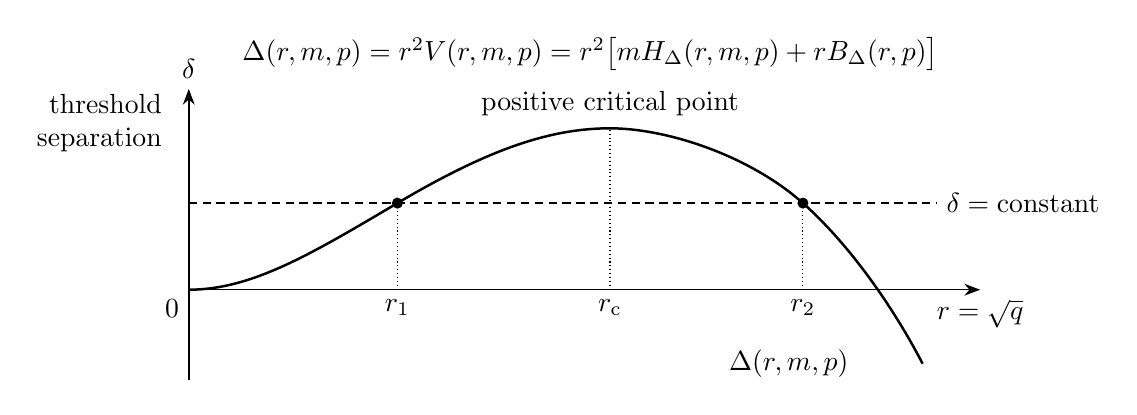
\begin{tikzpicture}[x=1cm,y=1cm,font=\normalsize,
      axis/.style={line width=.55pt,-{Stealth[length=2mm]}},
      graph/.style={line width=.9pt},
      guide/.style={line width=.45pt,densely dashed},
      projection/.style={line width=.4pt,densely dotted}]
    \node at (5.1,3.0)
      {$\Delta(r,m,p)=r^2V(r,m,p)=r^2\bigl[mH_\Delta(r,m,p)+rB_\Delta(r,p)\bigr]$};

    \draw[axis] (0,-1.15) -- (0,2.55)
      node[above] {$\delta$};
    \node[anchor=east,align=right] at (-.22,2.12)
      {threshold\\separation};
    \draw[axis] (0,0) -- (10.05,0)
      node[below] {$r=\sqrt q$};
    \node[below left] at (0,0) {$0$};

    % The two selected intersections lie on this hand-drawn guide.
    \draw[graph]
      (0,0)
      .. controls (.8,0) and (1.55,.45) .. (2.65,1.1)
      .. controls (3.75,1.75) and (4.55,2.05) .. (5.35,2.05)
      .. controls (6.05,2.05) and (7.1,1.72) .. (7.8,1.1)
      .. controls (8.45,.52) and (9.0,-.32) .. (9.32,-.94);
    \node[anchor=east] at (8.5,-.94) {$\Delta(r,m,p)$};

    \draw[guide] (0,1.1) -- (9.5,1.1)
      node[anchor=west] {$\delta=\text{constant}$};
    \draw[projection] (2.65,0) -- (2.65,1.1);
    \draw[projection] (7.8,0) -- (7.8,1.1);
    \draw[projection] (5.35,0) -- (5.35,2.05);
    \fill (2.65,1.1) circle[radius=2pt];
    \fill (7.8,1.1) circle[radius=2pt];
    \node[below] at (2.65,0) {$r_1$};
    \node[below] at (7.8,0) {$r_2$};
    \node[below] at (5.35,0) {$r_{\rm c}$};
    \node[above] at (5.35,2.08) {positive critical point};
  \end{tikzpicture}
  \caption{The separation graph $\delta=\Delta(r,m,p)$ for fixed $(m,p)$ with
    $c_0<0$, $A>0$ and $m>0$ (schematic). The graph has at most one positive
    critical point, which is nondegenerate
    (Proposition~\ref{prop:one-fold-graph}). Its intersections with a
    horizontal line are the zeros of $P''$ in the outer region $q>L|\delta|$,
    by~\eqref{eq:curvature-factor}; for other parameters the graph can be
    monotone. The resulting bound on fixed points is
    Proposition~\ref{prop:common-count}.}
  \label{fig:curvature-graph}
\end{figure}



\subsection{Attainment of the bounds}\label{subsec:single-scale-sharpness}

To attain six fixed points we choose a quartic with four simple positive
roots; its coefficients determine a quadratic with two simple negative roots.
We continue the two groups of roots in disjoint state intervals and then
treat the slices \(m=0\) and \(\delta=0\).

Assume~\eqref{eq:rank} and use the standard unfolding
\(\lambda=\Lambda(a,b,m,\delta)\) of Section~\ref{sec:introduction}, with
\(\lambda_0=\Lambda(0,0,0,0)\). Write
\[
 A_0=A_1(\lambda_0),\quad
 c_0=\tfrac12R_{\lambda_0}''(0),\quad
 B=|A_0|,\quad C=|c_0|,
\]
\[
 s=-\sgn c_0,\qquad \tau=\sgn(sA_0).
\]
We first allow an arbitrary rescaled strength sum, including zero:
\begin{equation}\label{eq:weighted-general-controls}
 \lambda_\eps=\Lambda(\bar a\eps^4,\bar b\eps^2,
                         \bar m\eps,\bar d\eps^3),\qquad
 \theta=(\bar a,\bar b,\bar m,\bar d),\qquad \eps>0.
\end{equation}

\begin{lemma}[Rescaled displacement]\label{lem:weighted-quartic}
Let \(\Omega_+\Subset(0,\infty)\), \(\Omega_-\Subset(-\infty,0)\), and let
\(\theta\) range over a fixed compact set. For sufficiently small
\(\eps>0\), the rescaled displacements satisfy, for \(z\in\Omega_+\)
and \(x\in\Omega_-\),
\begin{align}
 \mathcal F_\eps(z)&:=\eps^{-4}D_{\lambda_\eps}(\eps^2z^2)
 =F_\theta(z)+\eps E_+(\eps,z,\theta),\label{eq:quartic-limit}\\
 F_\theta(z)&=\bar a+\bar bz^2+\bar mz^3+c_0z^4+\tfrac32A_0\bar dz,\notag\\
 \mathcal G_\eps(x)&:=\eps^{-4}D_{\lambda_\eps}(\eps^2x)
 =G_\theta(x)+\eps E_-(\eps,x,\theta),
 \label{eq:quartic-negative-limit}\\
 G_\theta(x)&=\bar a+\bar bx+c_0x^2.\notag
\end{align}
The remainders extend jointly smoothly to signed \(\eps\) near zero.
For every prescribed finite integer \(n\), uniformly on these compacts,
\begin{equation}\label{eq:quartic-mixed-norm}
 \max_{j+|\gamma|\le n}
 \left\|\partial_z^j\partial_\theta^\gamma
                 (\mathcal F_\eps-F_\theta)\right\|_\infty\le C_n\eps,
\end{equation}
and similarly with \(x,\mathcal G_\eps\). The compact parameter set may
contain points with \(\bar m=0\).
\end{lemma}

\begin{proof}
Use the exact identities of Lemma~\ref{lem:exact-value-division}.
Substitute \(r=\eps z\), \(v=\bar d\eps/z^2\) into
\eqref{eq:quartic-Hadamard}; the profiles are evaluated at
\(\delta=r^2v=\bar d\eps^3\). Then
\[
 Q-q=\eps^4\Xi,\qquad
 \Xi=\bar mz^3+\bar dzH+\eps z^5L_0+\tfrac34\bar m^2\eps^2z^4.
\]
With \(Y=z^2+\eps^2\Xi\), the closing expansion gives
\begin{equation}\label{eq:quartic-exact-residual}
 \mathcal F_\eps=
 \bar a+\bar bY+\Xi+c(\lambda_\eps)Y^2
                   +\eps^2Y^3S(\eps^2Y,\lambda_\eps).
\end{equation}
Since \(z\) stays away from zero, all arguments remain in the common
root box, whose positive square-root factor stays bounded away from zero.
At \(\eps=0\), \(H=3A_0/2\) and \(c=c_0\), giving \(F_\theta\).
Taylor integral division in \(\eps\) proves the joint remainder and
every finite mixed estimate in \eqref{eq:quartic-mixed-norm}, without
dividing by \(\bar m\). State derivatives are taken at fixed
\((\eps,\theta)\), hence at fixed \(\lambda_\eps\); the variable
\(v=\bar d\eps/z^2\) keeps the separation \(r^2v=\bar d\eps^3\) fixed.

For negative \(x\) in a fixed compact set, \(q=\eps^2x\) is below
both thresholds for small positive \(\eps\), since \(\delta=O(\eps^3)\) and
\(|a_\delta|\le2|\delta|\). Thus \(Q=q\) exactly, and
\eqref{eq:quartic-closing-division} gives
\[
 \mathcal G_\eps=\bar a+\bar b x+c(\lambda_\eps)x^2
                   +\eps^2x^3S(\eps^2x,\lambda_\eps).
\]
This proves the negative formula and its joint smooth extension.
\end{proof}

For the six-point construction specialize to
\(\bar a=s\alpha_4\), \(\bar b=s\bsc\), \(\bar m=s\) and
\(\bar d=\tau\dsc\), giving
\begin{equation}\label{eq:quartic-weights}
 m=s\eps,\qquad \delta=\tau \dsc\eps^3,\qquad
 b=s\bsc\eps^2,\qquad a=s\alpha_4\eps^4,\qquad \eps>0.
\end{equation}
Here \(\alpha_4,\bsc,\dsc\) are rescaled parameters.
Multiplying the rescaled displacements by \(s\), and using
\(s\tau A_0=B\), \(sc_0=-C\), gives
\(\mathcal F_{4,\eps}:=s\mathcal F_\eps=F_0+O(\eps)\) and
\(\mathcal G_{4,\eps}:=s\mathcal G_\eps=G_0+O(\eps)\), where
\[
 \begin{aligned}
 F_0(z)&=\alpha_4+\bsc z^2+z^3-Cz^4+\tfrac32B\dsc z,\\
 G_0(x)&=\alpha_4+\bsc x-Cx^2.
 \end{aligned}
\]
These expansions have all the mixed estimates of
Lemma~\ref{lem:weighted-quartic}.

Take distinct positive numbers \(r_i\), \(1\le i\le4\), with
\(\sum r_i=1/C\), and let \(e_j\) be their elementary symmetric
functions. Choosing
\begin{equation}\label{eq:quartic-Vieta}
 \alpha_4=-Ce_4,\qquad \bsc=-Ce_2,\qquad \dsc=\frac{2C}{3B}e_3
\end{equation}
gives simultaneously
\[
 F_0(z)=-C\prod_{i=1}^4(z-r_i),\qquad
 G_0(x)=-C(x^2+e_2x+e_4).
\]
The six pair products have product \(e_4^3\); AM--GM yields
\(e_2\ge6\sqrt{e_4}\). Thus \(e_2^2-4e_4>0\), and the quadratic
has two distinct negative roots. Hence the choice~\eqref{eq:quartic-Vieta}
gives four simple positive roots of \(F_0\) and two simple negative roots
of \(G_0\).

\begin{proposition}[Six fixed points]
\label{prop:single-scale-six}
For every admissible family satisfying \eqref{eq:rank}, the standard
unfolding has six simple fixed points of order $\eps^2$ for all parameters
\eqref{eq:quartic-weights} with rescaled parameters in an open set and all
sufficiently small $\eps>0$. Their stability alternates: three are attracting
and three repelling.
\end{proposition}

\begin{proof}
Choose any distinct positive $r_i$ with sum $1/C$ and the parameters
\eqref{eq:quartic-Vieta}. The four roots of $F_0$ and the two negative
roots of $G_0$ have strict derivative margins. Lemma~\ref{lem:weighted-quartic}
continues them on six disjoint isolating intervals, uniformly over a small
open set of rescaled parameters. The same joint estimates allow \(\bar m\) to
vary near \(s\), so this set may be taken open in all four rescaled
parameters. Fixed rescaled parameters give a smooth parameter path tending to
the reference, and Proposition~\ref{prop:common-count} excludes additional
fixed points. At these parameters, for negative states $D_q=s\eps^2G_0'(x)+O(\eps^3)$, and for positive
states $D_q=s\eps^2F_0'(z)/(2z)+O(\eps^3)$. In state order these signs
are $s(+,-,+,-,+,-)$. Since the return is increasing and close to the
identity, they give three attracting and three repelling hyperbolic cycles;
these signs persist on the open set of rescaled parameters.
\end{proof}

\begin{proposition}[Attainment on the slices]
\label{prop:sharp-slice-attainment}
For every admissible family satisfying \eqref{eq:rank}, the standard unfolding
has four simple fixed points on \(\delta=0\), four on \(m=0\), and two on
\(m=\delta=0\). Each configuration occurs in \(I\) for every sufficiently
small \(\eps>0\) along a smooth parameter path tending to the reference, and
persists on an open set of rescaled parameters within the corresponding slice.
\end{proposition}

\begin{proof}
Use the weights \eqref{eq:weighted-general-controls}. The following table
specifies the paths and the limiting simple roots; positive roots use the
coordinate $z$, and negative roots the coordinate $x$:
\begin{equation}\label{eq:sharp-slice-controls}
 \begin{array}{c|c|c|c}
 \text{slice}&(\bar a,\bar b,\bar m,\bar d)/(sC)&z>0&x<0\\ \hline
 \delta=0&(36/11,-85/11,60/11,0)&1,2,3&x_\delta\\
 m=0&(36,25,0,-40/A_0)&1,2,3&x_m\\
 m=\delta=0&(1,0,0,0)&1&-1
 \end{array}
\end{equation}
Here $x_\delta=(-85-\sqrt{8809})/22$ and
$x_m=(25-\sqrt{769})/2$. For the first two rows, direct substitution in
Lemma~\ref{lem:weighted-quartic} gives respectively
\[
 \begin{aligned}
 F_\theta/(sC)&=-(z-1)(z-2)(z-3)(z+6/11),&
 G_\theta/(sC)&=36/11-85x/11-x^2,\\
 F_\theta/(sC)&=-(z-1)(z-2)(z-3)(z+6),&
 G_\theta/(sC)&=36+25x-x^2.
 \end{aligned}
\]
Only the positive roots of $F_\theta$ correspond to fixed points; the
negative ones come from $G_\theta$. The estimates of
Lemma~\ref{lem:weighted-quartic} include $\bar m=0$.

For the third row, \eqref{eq:center-displacement} and the root-profile
remainder estimates give, uniformly on compact $x$-intervals including zero,
\[
 \frac{D_{\lambda_\eps}(\eps^2x)}{sC\eps^4}
 =1-x^2+O_{C^1}(\eps).
\]

Continue the listed simple roots by Lemma~\ref{lem:weighted-quartic} and
the isolating argument in the proof of Proposition~\ref{prop:single-scale-six}
on small relatively open sets of rescaled parameters with compact closures:
$\bar d=0$ in the first row, $\bar m=0$ in the second, and $\bar m=\bar d=0$
with $(\bar a,\bar b)$ near $(sC,0)$ in the third. The rescaled thresholds
are $0$ and $a_\delta/\eps^2$, with
$|a_\delta|/\eps^2\le2|\bar d|\eps$. One reduction of
$\eps$ places the positive intervals where both passages are active, the
negative ones below both thresholds, the parameters in the domain of
$\Lambda$, and the rescaled intervals in $I$.
Corollary~\ref{cor:four-slices} excludes other roots in $I$, including at the
thresholds, and $\Lambda$ gives smooth parameter paths and relative
persistence.
\end{proof}

The positive quartet in the six-cycle construction is the starting point for
Section~\ref{sec:main-saturation}.

\section{The saturation domain at the principal scale}\label{sec:main-saturation}
\label{sat:section}

The saturation domain has a limiting geometry described by a quartic with
four nonnegative roots. For a return with six fixed points, we first derive
the weights of the parameters and of the fixed points from the five
alternating extrema of its displacement. Estimates near the thresholds then
control critical points that
approach the thresholds, and their limiting values determine the four-root
region. The necessary estimates hold in every admissible family. We prove the
weights introduced in Section~\ref{sec:introduction}, beginning with
a tail estimate that converts weighted parameter bounds into bounds on the
fixed points.

\begin{lemma}[A tail bound from weighted parameters]\label{mainloc:tail}
For every fixed $K_0>0$, there are common constants $M,m_0>0$ such
that, whenever $0<|m|<m_0$ and
\[
 |a|\le K_0m^4,\qquad |b|\le K_0m^2,\qquad
 |\delta|\le K_0|m|^3,
\]
every zero of $D$ in $I$ satisfies $|q|<Mm^2$. On the two complementary
tails, $D$ has the sign of $c$.
\end{lemma}

\begin{proof}
Let $0<q_{\mathrm{in}}<q_0$ be an inner radius, to be fixed below.
For $Mm^2\le q\le q_{\mathrm{in}}$, reduce $m_0$ so that
$|\delta|/q\le K_0|m|/M\le1$. Equation~\eqref{eq:quartic-global-value}
gives
\[
 \frac{|Q-q|}{q^2}\le K\{M^{-1/2}+M^{-3/2}+m^2+\sqrt{q_{\mathrm{in}}}
                                      +m^2M^{-1/2}\}.
\]
In particular, the strength-sum and separation terms use respectively
$|m|/\sqrt q\le M^{-1/2}$ and
$|\delta|\sqrt{q+|\delta|}/q^2\le KM^{-3/2}$.
For small $q_{\mathrm{in}}$, this also gives $|Q-q|/q<1/2$. The closing
expansion yields
\[
 D-cq^2=a+bq+(1+b)(Q-q)
       +c\{2q(Q-q)+(Q-q)^2\}+Q^3S(Q,\lambda).
\]
Consequently
\begin{equation}\label{sat:tail-estimate}
 \frac{|D(q)-c(\lambda)q^2|}{q^2}
 \le K\{M^{-2}+M^{-1}+M^{-1/2}+M^{-3/2}
                              +\sqrt{q_{\mathrm{in}}}+|m|\}.
\end{equation}
The first two terms bound $a/q^2$ and $b/q$; the remaining closing
terms follow from $|Q|\le2q$ and the bound for $Q-q$.
For $-q_{\mathrm{in}}\le q\le-Mm^2$, both passage inputs are negative once $m_0$ is
small: $q<\min(0,\delta)$. Thus $Q=q$ exactly, and the same estimate
follows directly from the closing expansion. Choose $M$ large, then
$q_{\mathrm{in}}$ small and $m_0$ small so that the right-hand side is less than
half the common lower bound for $|c|$; reduce $m_0$ further so that
$Mm_0^2<q_{\mathrm{in}}$.

The rest of the original common interval $I=(-q_0,q_0)$ is covered as
follows. At the reference, \eqref{eq:center-displacement}
gives $D(0)=D'(0)=0$ and strict curvature of sign $c_0$ throughout
the reduced interval. Hence $D$ has that sign at every
nonzero reference state. The closed outer state set
$q_{\mathrm{in}}\le |q|\le q_0$ is compact and has a nonzero value margin; joint continuity in the
parameters preserves it after one common parameter reduction. The common domains are chosen to contain
$\overline I$, so this argument covers the whole interval.
All choices are made before any parameter path is chosen.
\end{proof}

\begin{lemma}[Returns with six fixed points]
\label{sat:saturation}\label{corner:saturated-geometry}
\label{cor:six-necessary-window}
If $D$ has six zeros in $I$, then
\[
 mc_0(p)<0,\qquad \delta A(p)c_0(p)<0,\qquad
 0<\delta/\delta_{\rm c}(m,p)<1.
\]
In particular $0<|\delta|<|\delta_{\rm c}|\le K|m|^3$ uniformly.
Put $s=-\sgn c_0$, $E=sD$, and denote the thresholds by $\theta_1<\theta_2$.
Then $P''$ has two simple zeros $\zeta_1<\zeta_2$ in the outer region, and
\begin{equation}\label{sat:curvature-signs}
 \begin{array}{c|ccccc}
 q&(-q_0,\theta_1)&(\theta_1,\theta_2)&(\theta_2,\zeta_1)&
       (\zeta_1,\zeta_2)&(\zeta_2,q_0)\\ \hline
 \sgn E''&-&+&-&+&-
 \end{array}
\end{equation}
The continuous $E'$ has exactly one zero in each open interval, none
at its shared junctions, and
\begin{equation}\label{sat:junction-slopes}
 E'(\theta_1)<0,\quad E'(\theta_2)>0,\quad
 E'(\zeta_1)<0,\quad E'(\zeta_2)>0.
\end{equation}
All six zeros are simple $C^1$ zeros, including any at a threshold.
The extremal values have signs $+,-,+,-,+$; the first is an inactive
positive maximum and the second a negative minimum between the thresholds.
On $\delta=\delta_{\rm c}$, $mc_0<0$, there are at most four fixed points.
\end{lemma}

\begin{proof}
The four-point slices exclude $m=0$ and $\delta=0$.
The signs~\eqref{eq:event-signs} give the number
$s_E=1+\mathbf1_{\{\delta Ac_0<0\}}$ of curvature sign changes at the thresholds.
Let $s_O\le2$ be the number of sign changes at zeros of $P''$ in the outer
region. Joining same-sign pieces through isolated zeros and thresholds gives at most $s_E+s_O+1\le5$
strict monotonicity blocks for the continuous $D'$. Each block,
with its finite endpoints, contains at most one zero. Six zeros of
$D$ give five distinct derivative zeros in their open gaps by $C^1$
Rolle, so $s_E=s_O=2$. Proposition~\ref{prop:cubic-curvature-window}
gives the stated window and cubic bound. The signs~\eqref{eq:event-signs} and the outer
factorization~\eqref{eq:curvature-factor} give~\eqref{sat:curvature-signs}.

Retain every shared finite junction in both adjacent blocks of $E'$.
A derivative zero there would occupy both blocks, leaving room for at
most four distinct derivative zeros. Hence all five lie in the five
respective interiors, and strict monotonicity gives
\eqref{sat:junction-slopes}. A stationary fixed point would supply a
sixth derivative zero distinct from the five open-gap zeros. Thus none
occurs, including at a threshold.
The extrema interlace the six roots, giving all five strict value signs.
At $\delta=\delta_{\rm c}$ the double zero of $P''$ does not change sign, leaving at most three blocks and four distinct fixed
points. Truncating at the ends of the common interval removes blocks
but cannot add them.
\end{proof}

\begin{proposition}[Weighted confinement]
\label{sat:weighted-confinement}
For every admissible family there are a further reduction of \(I\) and
\(U\) and a constant \(K>0\) with the following property. If \(P_\lambda\)
has six fixed points \(q_1,\ldots,q_6\) in \(I\), then
\begin{equation}\label{sat:weighted-bounds}
 0<|\delta|\le K|m|^3,\qquad
 |b|\le K|m|^2,\qquad |a|\le K|m|^4,\qquad
 \max_j|q_j|\le K|m|^2.
\end{equation}
\end{proposition}

\begin{proof}
We use the auxiliary-control convention following
Lemma~\ref{lem:auxiliary-controls} also when \(m\) and \(\delta\) are dependent.
The jets \(a,b\) are those of~\eqref{eq:regular-jets}.

Lemma~\ref{cor:six-necessary-window} already gives the first
bound in \eqref{sat:weighted-bounds}. At a curvature zero write
\(q=r^2\). The exact division \eqref{eq:V-division} gives
\begin{equation}\label{sat:curvature-state}
 \delta=r^2\{mH_\Delta(r,m,p)+rB_\Delta(r,p)\}.
\end{equation}
Here \(H_\Delta\) has sign \(A\), and \(B_\Delta\) has sign \(c_0/A\),
with uniform nonzero margins. In the sign case forced by six zeros,
\(mH_\Delta\) has the sign of \(\delta\), whereas \(rB_\Delta\) has the
opposite sign. Equation~\eqref{sat:curvature-state} consequently
implies
\begin{equation}\label{sat:curvature-scale}
 r\le K|m|,\qquad
 |v|=|\delta|/r^2=|mH_\Delta+rB_\Delta|\le K|m|
\end{equation}
at both zeros of \(P''\).

The derivative \(Q'\), taken at fixed parameters,
has the smooth root expression \eqref{eq:Q-outer}. It equals one
at \(r=0\), so \(Q'-1=rU_1(r,m,v,p)\) with \(U_1\) smooth.
The aligned strength cancellation gives \(U_1(0,0,0,p)=0\).
Hence
\begin{equation}\label{sat:outer-slope-bound}
 |Q'-1|\le K r(r+|m|+|v|).
\end{equation}
At \(\zeta_2\), equations~\eqref{sat:curvature-scale} and
\eqref{sat:outer-slope-bound}, together with \(Q=O(r^2)\), yield
\(D'(\zeta_2)=b+O(m^2)\). At the first threshold \(Q'=1\).
For positive separation that threshold is zero and \(Q=0\), giving
\(D'(\theta_1)=b\); for negative separation it is \(\delta\), with
\(Q=\delta\), giving \(D'(\theta_1)=b+O(|\delta|)\).
The first and last inequalities in \eqref{sat:junction-slopes}
therefore imply
\[
 -Km^2\le sb\le K|\delta|.
\]
The cubic separation bound proves \(|b|\le K|m|^2\).

For the offset and the states, use the bound
\eqref{eq:quartic-global-value}, which is uniform up to the thresholds.

On the inactive side the exact closing expansion gives
\[
 E(q)=sa+sbq+sc(\lambda)q^2+O(|q|^3).
\]
After shrinking the state interval, its last two terms are bounded
above by \(-\gamma q^2\) for one \(\gamma>0\). Completing the
square gives \(E(q)\le sa+Kb^2\). The positive inactive maximum
from Lemma~\ref{sat:saturation} therefore implies
\begin{equation}\label{sat:offset-lower-coarse}
 sa\ge-Kb^2.
\end{equation}
The next, negative minimum lies between the two thresholds, where
\(|q|\le K|\delta|\). Equation~\eqref{eq:quartic-global-value} and the
closing expansion give there
\[
 |D(q)-a|\le K\{ |b\delta|+|\delta|^{3/2}+\delta^2\}.
\]
Consequently
\begin{equation}\label{sat:offset-upper-coarse}
 sa\le K\{ |b\delta|+|\delta|^{3/2}+\delta^2\}
       \le K|m|^{9/2}.
\end{equation}
Together with \eqref{sat:offset-lower-coarse}, this proves
\(|a|\le K|m|^4\).

The three parameter bounds just proved satisfy the hypotheses of
Lemma~\ref{mainloc:tail}, which confines every zero to $|q|<Mm^2$.
\end{proof}

\subsection{The four-root limit}\label{subsec:four-root-limit}

The parameter and state weights are now forced by the six-point
configuration. We next identify the coefficient geometry of its limits.

Fix the sign case $A_1(\lambda_0)=B>0$ and $c_0=-C<0$, and define
\[
 A_4=C^3a/m^4,\qquad S_4=-Cb/m^2,\qquad
 T_4=3BC^2\delta/(2m^3),\qquad x=C\sqrt q/m.
\]
Here $B$ and $C$ are reference values. Write
\[
 \Phi_{A,S,T}(x)=A-Sx^2+x^3-x^4+Tx,
 \qquad
 \mathcal K_4=\{(-e_4(r),e_2(r),e_3(r)):r_i\ge0,\ \sum_i r_i=1\}.
\]

Let $\Lambda$ be the standard unfolding, defined on a neighbourhood
$\mathcal V\subset\mathbb R^4$ of $0$. Write
\[
 N_\lambda(I)=\#\{q\in I:D_\lambda(q)=0\},\qquad
 v_m(A,S,T)=\left(\frac{m^4A}{C^3},-\frac{m^2S}{C},m,
                         \frac{2m^3T}{3BC^2}\right).
\]
Choose a compact box $\mathcal B$, independent of $m$, containing
$\mathcal K_4$ in its interior and the normalized parameters of every
six-cycle configuration in $\mathcal V$;
Proposition~\ref{sat:weighted-confinement} provides such a box after
shrinking $\mathcal V$. Define
\begin{equation}\label{def:actual-main-domain}
 \mathscr T_m=\{(A,S,T)\in\mathcal B:v_m(A,S,T)\in\mathcal V,
                    N_{\Lambda(v_m(A,S,T))}(I)=6\}.
\end{equation}

For $x>0$ put $F_m(x)=C^3m^{-4}D(m^2x^2/C^2)$. At fixed parameters,
\[
 D_q=\frac{m^2}{2Cx}F_m',\qquad
 D_{qq}=\frac{C}{4x^3}(xF_m''-F_m').
\]
Thus the limiting curvature equation is
$x\Phi''-\Phi'=3x^2-8x^3-T=0$, with positive critical point $x=1/4$,
critical value $T=1/16$, and nonzero root $x=3/8$ when $T=0$.

\begin{lemma}[Convergence at the principal scale]\label{lem:k4-sequence}
Let parameters tend to the reference, let $m>0$ tend to zero, and assume
that $(A_4,S_4,T_4)$ stays bounded. If these triples converge to $(A,S,T)$,
then
\[
 \frac{C^3}{m^4}D(m^2x^2/C^2)\longrightarrow\Phi_{A,S,T}(x)
\]
in $C^k$ on every compact subset of $x>0$, for every fixed finite $k$.
\end{lemma}
\begin{proof}
Put $r=mx/C$ and $v=\delta/r^2=2mT_4/(3Bx^2)$. On a positive compact
$x$-interval, $r,m,v\to0$ uniformly with all fixed-order $x$ derivatives.
The division~\eqref{eq:actual-both-active-division} gives
\[
 Q-q=mr^3+\tfrac34m^2r^4+r^5L_0+\delta rH,
 \qquad H(0,0,0,p)=\tfrac32A_1(p,0,0).
\]
Consequently $C^3(Q-q)/m^4\to x^3+Tx$ in every such $C^k$ norm.
In the closing expansion
\[
 D=a+bQ+(Q-q)+c(\lambda)Q^2+Q^3S_R,
\]
we have $Q=q+O_{C^k}(m^4)$, $b=-m^2S_4/C$, and $c(\lambda)\to-C$.
The four remaining terms therefore converge respectively to
$A$, $-Sx^2$, $-x^4$, and zero after multiplication by $C^3/m^4$.
All profiles are evaluated in one compact neighbourhood, so their state
derivatives are controlled however the remaining parameters converge.
\end{proof}

Convergence on positive compact intervals leaves open the behaviour near
the thresholds. The next lemma controls the critical point that can collapse
onto a threshold.

\begin{lemma}[Critical points near the thresholds]\label{lem:k4-event}
Let parameters tend to the reference through returns with six fixed points,
and let their normalized coefficients converge to $(A,S,T)$. Denote the five successive critical points of $D$
by $t_1,\ldots,t_5$, and put $x_j=C\sqrt{t_j}/m$ for $j=3,4,5$.
If $T>0$, all three $x_j$ stay in a compact subset of $(0,\infty)$.
If $T=0$, then $x_3\to0$, $A=0$, and every limit of $x_5$ is at least
$3/8$.
\end{lemma}
\begin{proof}
The critical points interlace the six zeros, so their upper bounds follow
from the state confinement in \eqref{sat:weighted-bounds}. The offset
estimate~\eqref{sat:offset-upper-coarse} gives
$a\le K m^{9/2}$, hence $A\le0$.

Suppose first that $T>0$ and that $x_3\to0$ along a subsequence.
At $q=t_3$ both passages are active. Let $y=\Gamma_1(q)-\delta\ge0$.
Since $q^{3/2}/\delta$ is a fixed positive constant times $x_3^3/T_4$,
this ratio tends to zero. More generally, on the common small parameter
and state domain, assume $A_1\ge B/2$, $m>0$, $\delta>0$, $q>0$ and
$y\ge0$. If $q^{3/2}/\delta$ is sufficiently small, the passage value
estimate gives
\[
 q-y\ge\delta/2,\quad 0\le y<q,\quad
 \sqrt q-\sqrt y\ge\delta/(4\sqrt q).
\]
The derivative expansion, with all coefficients evaluated at the same
parameter, is
\[
 Q_q-1=\tfrac32A_1(\sqrt q-\sqrt y)
       +\tfrac32(A_1+A_2)\sqrt y+O(q).
\]
The strength identity gives $A_1+A_2=m>0$. Also $Q=O(q)$,
$Q_q=1+O(\sqrt q)$, and $R'(Q)-1=b+O(q)$. Consequently, for common
constants $\kappa,K>0$,
\begin{equation}\label{sat:threshold-slope-exclusion}
 D_q(q)\ge \kappa\delta/\sqrt q-K(|b|+q).
\end{equation}
This estimate includes $y=0$, the second threshold, by continuity of the
passage derivatives. Applied at $t_3$ and multiplied by $C/m^2$, its
right-hand side is bounded below by
$\kappa_1T_4/x_3-K_1-K_2x_3^2$, which tends to $+\infty$. This contradicts
$D_q(t_3)=0$. The ordering $x_3<x_4<x_5$ proves the first assertion.

Now suppose $T=0$. Write $r_-<r_+$ for the square roots of the two zeros
of $P''$ in the outer region. They lie on opposite sides of the unique
positive critical point $r_{\rm c}$ of the separation graph. Its exact
formula~\eqref{sat:curvature-state} and the boundary coefficients in
\eqref{eq:B-boundary}--\eqref{eq:V-division} give, for bounded $x=Cr/m$,
\[
 T_4=3x^2-8x^3+o(1),\qquad Cr_{\rm c}/m\longrightarrow1/4.
\]
The error is uniform down to $x=0$ because the graph profiles are smooth.
Both $Cr_\pm/m$ are bounded by the curvature-zero confinement
\eqref{sat:curvature-scale}. A limit
of $Cr_-/m$ lies in $[0,1/4]$ and solves $x^2(3-8x)=0$, hence is zero.
A limit of $Cr_+/m$ is at least $1/4$ and solves the same equation, hence
is $3/8$. Since $t_3<r_-^2$ and $t_5>r_+^2$, the location assertions follow.

The estimate~\eqref{eq:quartic-global-value} yields
\[
 |D(q)-a|\le K\{|b|q+q^2+mq^{3/2}+m^2q^2+q^{5/2}
                +\delta\sqrt{q+\delta}+\delta q^{3/2}\}.
\]
At $q=t_3$, division by $m^4$ bounds this by a constant times
\[
 x_3^2+x_3^3+x_3^4+m^2x_3^4+mx_3^5
 +T_4x_3+\sqrt m\,T_4^{3/2}+m^2T_4x_3^3,
\]
which tends to zero. Since $D(t_3)>0$, this gives $A\ge0$, and therefore
$A=0$.
\end{proof}

These two convergence statements allow the critical-value signs to pass
to the quartic, including its zero-root face.

\begin{proposition}[Necessary four-root geometry]\label{prop:k4-necessary}
In this sign case, for every admissible family, every accumulation point of
$(A_4,S_4,T_4)$ along a saturated sequence belongs to $\mathcal K_4$.
\end{proposition}
\begin{proof}
Take a convergent coefficient subsequence, using \eqref{sat:weighted-bounds}.
In this sign case \eqref{sat:junction-slopes} gives $b=D'(0)<0$ on every
saturated return, so $S_4=-Cb/m^2>0$ and its limit satisfies $S\ge0$.
If $T>0$, Lemmas~\ref{lem:k4-sequence} and~\ref{lem:k4-event} give three
positive limiting critical points $u\le v\le w$ of $\Phi$, with
\[
 \Phi(u)\ge0,\qquad\Phi(v)\le0,\qquad\Phi(w)\ge0.
\]
If $k\le3$ critical points converge to the same positive point $z$,
repeated Rolle gives zeros of $F_m^{(j)}$ tending to $z$ for
$1\le j\le k$. The $C^3$ convergence yields $\Phi^{(j)}(z)=0$ for
those $j$, so $z$ is a zero of $\Phi'$ of multiplicity at least $k$.
If $u<v<w$, the four successive intervals
$[0,u],[u,v],[v,w],[w,\infty)$ each contain a zero, since $\Phi(0)=A\le0$
and $\Phi$ tends to $-\infty$. A zero at a shared critical endpoint has
multiplicity at least two, so the four interval allocations are valid
when counted with multiplicity. If $u=v<w$, then $\Phi(u)=0$ and the
double derivative zero gives a triple polynomial zero at $u$; a fourth
zero lies in $[w,\infty)$. The case $u<v=w$ is analogous. If all three
merge, the common value is zero and the root has multiplicity four.
Thus all four roots are nonnegative and their sum is one.

If $T=0$, Lemma~\ref{lem:k4-event} gives $A=0$. After subselection $x_5\to w\ge3/8$,
and positive-compact convergence gives $\Phi(w)\ge0$. Therefore
$-S+w-w^2\ge0$, so $0\le S\le1/4$. The factorization
$\Phi=x^2(-x^2+x-S)$ again gives four nonnegative roots with sum one.
\end{proof}

\begin{proof}[Completion of Theorem~\ref{thm:main-saturation-summary}]
The interior of $\mathcal K_4$ consists exactly of coefficient triples
with four distinct positive roots. The set of such triples is open by simple-root
continuation. A zero root or a multiple root is a boundary point: a
small constant-term perturbation gives respectively a negative root or
violates one of the necessary critical-value signs for four real roots.
Triples with distinct positive roots are dense, by perturbing the root
vector inside the simplex while preserving its sum.

For positive roots $r_i$ of an interior triple, the construction in the
proof of Proposition~\ref{prop:single-scale-six} with $r_i/C$ and $\eps=m$
gives exactly the parameters $v_m(A,S,T)$ and two simple negative roots. On
each compact subset of the interior, uniform isolation and nonzero derivative
margins let Lemma~\ref{lem:weighted-quartic} continue all six roots in the
standard unfolding for uniformly small $m>0$; Proposition~\ref{prop:common-count}
excludes others in $I$.

For the Hausdorff upper inclusion, a contrary sequence of closure points
can be approximated within $1/n$ by true points of $\mathscr T_{m_n}$.
Compactness of $\mathcal B$ and Proposition~\ref{prop:k4-necessary} then
force its limit into $\mathcal K_4$. For the lower inclusion, approximate
compact $\mathcal K_4$ by a finite net of interior points and realize all
of them at every sufficiently small $m$.
\end{proof}

\subsection{Boundary geometry of the limiting domain}

Figure~\ref{fig:main-saturation-sections} displays two sections of the
limiting coefficient region; the critical-value criterion below describes
their boundaries.

\begin{figure}[!htbp]
\centering
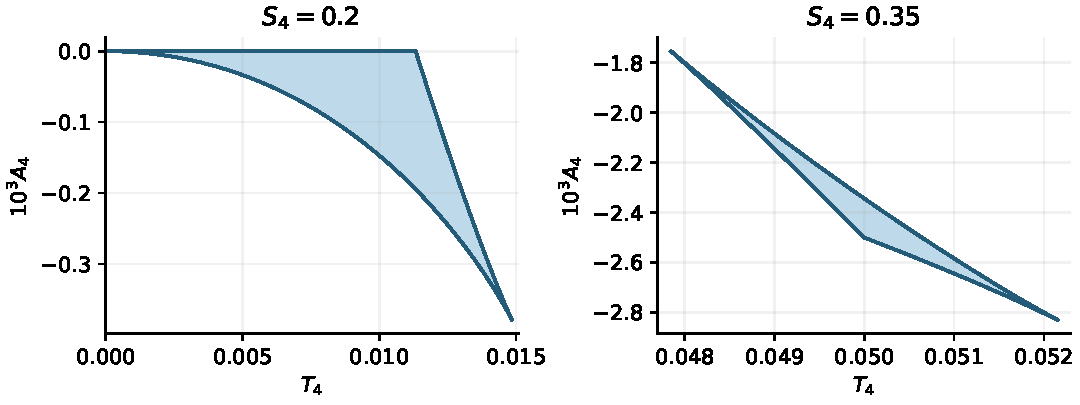
\includegraphics[width=\textwidth]{figures/main-saturation-sections.pdf}
\caption{Sections of the limiting four-root domain at $S_4=0.2$ and
$S_4=0.35$. The ordinate is $10^3A_4$, and the two panels have different
axis ranges. The boundaries are drawn from the critical-value interval
described below. In the left panel the segment $A_4=0$ represents a zero
root. The remaining boundary arcs have repeated roots; the two lower
bounds switch when $f(u)=f(w)$, where the two local maxima have equal value.}
\label{fig:main-saturation-sections}
\end{figure}

The symmetric mean inequalities give
\[
 -\frac1{256}\le A_4\le0,\qquad
 0\le S_4\le\frac38,\qquad 0\le T_4\le\frac1{16}.
\]
The three coefficient extrema $A_4=-1/256$, $S_4=3/8$,
and $T_4=1/16$ are attained at $r_i=1/4$, where
$\Phi=-(x-1/4)^4$. At the opposite face, $e_3=0$ forces at least two
roots to vanish, and therefore
\[
 \mathcal K_4\cap\{T_4=0\}
 =\{(0,S_4,0):0\le S_4\le1/4\}.
\]
These bounds are sharp for $\mathcal K_4$ and hold asymptotically along
saturated sequences.

For fixed $S_4,T_4$ with three positive critical points $u<v<w$, put
$f(x)=-S_4x^2+x^3-x^4+T_4x$. The admissible offset interval is
\[
 \max\{-f(u),-f(w)\}\le A_4\le\min\{0,-f(v)\}.
\]
It is nonempty precisely when these critical-value inequalities are
compatible. Taking closures includes merged critical points in this
description of the limiting boundary.

\section{Limit cycles of multiplicity four and their unfolding}
\label{sec:actual-bifurcations}

We continue the fourfold limiting root to a limit cycle of multiplicity four
for small $m>0$ and describe its unfolding together with the two simple fixed
points with $q<0$. We use the standard unfolding in the sign case
$A_1(\lambda_0)=B>0$, $c_0=-C<0$. The proof has three steps: location of all
zeros in $I$, including near the thresholds; construction of the multiple
root; and preparation of the positive cluster in a chart where $D$ is smooth
in $q$.

\begin{lemma}[Values across the thresholds]
\label{mainloc:cross-event}
Set
\begin{equation}\label{mainloc:weights}
 a=\frac{m^4A}{C^3},\qquad b=-\frac{m^2S}{C},\qquad
 \delta=\frac{2m^3T}{3BC^2},\qquad q=\frac{m^2\zeta}{C^2},
 \qquad m>0.
\end{equation}
For every compact set of $(A,S,T)$ and every bounded $\zeta$-interval,
uniformly on their product,
\begin{equation}\label{mainloc:full-limit}
 \frac{C^3}{m^4}D\left(\frac{m^2\zeta}{C^2}\right)
 =A-S\zeta-\zeta^2+\zeta_+^{3/2}
                 +T\sqrt{\zeta_+}+O(\sqrt m).
\end{equation}
This is a $C^0$ estimate, uniform across both thresholds.
\end{lemma}

\begin{proof}
Hold $a,b,m$ fixed and integrate in the separation $t$ from $0$
to $\delta$. Put $y=\Gamma_1(q,t)-t$. The passage
jet and its parameter derivatives give
\[
 \Gamma_{\nu,q}(x)=1+\tfrac32A_\nu\sqrt{x_+}+O(x_+),\qquad
 \Gamma_{\nu,t}(x)=O(x_+^{3/2}),\qquad
 |y-q|\le K(q_+^{3/2}+|t|).
\]
These estimates include zero inputs. Along the integration segment,
$A_2=-B+O(m)$ and $|t|=O(m^3)$. The square-root inequality
$|\sqrt{y_+}-\sqrt{q_+}|\le\sqrt{|y-q|}$ and the total derivative
\eqref{eq:quartic-total-detuning} therefore give
\begin{align*}
 \left|Q_t-\tfrac32B\sqrt{q_+}\right|
 \le K\{&q_+^{3/4}+\sqrt{|t|}+m\sqrt{q_+}+q_++|t|\\
        &+q_+^{3/2}+(q_++|t|)^{3/2}\}=O(m^{3/2}).
\end{align*}
This bound uses $|t|$ and remains valid for $q<0$, so both signs
of separation are included. Integration and the aligned identity
\eqref{eq:passage:aligned-jet} yield
\[
 Q-q=mq_+^{3/2}+\tfrac32B\delta\sqrt{q_+}+O(m^{9/2}),
 \qquad Q-q=O(m^4).
\]
In \eqref{eq:quartic-closing-division}, $c=-C+O(m)$ because the
remaining parameters are fixed at $\xi_0$. Replacing $Q$ by $q$
in $bQ+cQ^2$ changes these terms by $O(m^6)$, while
$(c+C)q^2=O(m^5)$ and $Q^3S=O(m^6)$. Thus
\[
 D=a+bq-Cq^2+mq_+^{3/2}
                    +\tfrac32B\delta\sqrt{q_+}+O(m^{9/2}).
\]
Substitution of \eqref{mainloc:weights} proves the assertion.
\end{proof}

With \eqref{mainloc:weights}, set $\Theta=(A,S,T)$ and
\begin{equation}\label{quartic:centre}
 \Theta_0=\left(-\frac1{256},\frac38,\frac1{16}\right),\qquad
 x_0=\frac14.
\end{equation}
To count cycles on both sides of this bifurcation, we first locate
all zeros near the fourfold configuration.

\begin{lemma}[All roots near the quadruple configuration]
\label{mainloc:all-roots}
There are a neighbourhood $\mathcal O$ of $\Theta_0$, $m_0>0$
and three disjoint compact state intervals $J_{N,-},J_{N,+},J_Q$
about, respectively,
\[
 \zeta_{N,\pm}=\frac{-3\pm2\sqrt2}{16}<0,\qquad
 \zeta_Q=\frac1{16}>0,
\]
such that, for every $\Theta\in\mathcal O$ and $0<m<m_0$, all zeros in
$I$ lie in $(m^2/C^2)(J_{N,-}\cup J_{N,+}\cup J_Q)$.
Each negative interval contains exactly one simple zero. Both passages are
active on the positive interval, which contains all remaining zeros.
The three intervals can be chosen arbitrarily small about their
respective centres, by reducing $\mathcal O$ and $m_0$.
\end{lemma}

\begin{proof}
Bounded parameters satisfy the hypotheses of Lemma~\ref{mainloc:tail}.
Thus all zeros have $|\zeta|\le L$ for a fixed $L$.
At $\Theta_0$, the full-state limit in
\eqref{mainloc:full-limit} is
\[
 -\left(\zeta-\zeta_{N,-}\right)
       \left(\zeta-\zeta_{N,+}\right)\quad(\zeta<0),\qquad
 -\left(\sqrt\zeta-\tfrac14\right)^4\quad(\zeta\ge0).
\]
Its only root positions are the three stated centres, and its value
at zero is $-1/256$. Choose the three small intervals with each centre
in its interval's interior. The complement of their interiors in
$[-L,L]$ is compact and contains no limiting root, so the absolute value
of the limiting function has a positive minimum there. First reducing
$\mathcal O$, then $m_0$, preserves that gap by
Lemma~\ref{mainloc:cross-event}. This excludes all zeros outside the interval
interiors, including their boundaries and the threshold layer.

Take $\mathcal O$ so that $T>0$. For $q<0$ both passages are inactive, so
the closing expansion gives on either negative interval
\[
 \frac{C^3}{m^4}D(m^2\zeta/C^2)
 =A-S\zeta-\zeta^2+O_{C^1}(m).
\]
The limiting derivatives at $\zeta_{N,-},\zeta_{N,+}$ are
$\sqrt2/4,-\sqrt2/4$. Their strict signs and the opposite endpoint
values persist uniformly. The intermediate value theorem and strict
monotonicity give one simple root in each interval. In particular,
their scaled locations are
\[
 \frac{-S\pm\sqrt{S^2+4A}}2+O(m).
\]
Finally the second threshold is
$a_\delta=\Gamma_1^{-1}(\delta)=O(m^3)$, whereas the positive interval
has $q\ge \kappa m^2$ for a fixed $\kappa>0$. Hence that entire interval
lies beyond both thresholds.
\end{proof}

The localization fixes the two negative zeros and places the positive
cluster beyond both thresholds. It remains to meet the four zero conditions
simultaneously and identify the local unfolding. The following theorem refines
Theorem~\ref{thm:actual-quartic-summary}.

\begin{theorem}[Limit cycles of multiplicity four]
\label{thm:actual-quartic}
After a reduction of $\mathcal O$ and $m_0$ in
Lemma~\ref{mainloc:all-roots}, there is a unique smooth branch
$m\mapsto(\Theta_*(m),x_*(m))$, $0\le m<m_0$, equal to $(\Theta_0,x_0)$ at
$m=0$, such that for every $0<m<m_0$ the displacement has a zero of
multiplicity four at $q_*(m)=m^2x_*(m)^2/C^2$ for the parameters
$\Theta_*(m)$. Its parameters and state satisfy
\begin{equation}\label{quartic:physical-branch}
 \begin{aligned}
 a_*(m)&=-\frac{m^4}{256C^3}+O(m^5),&
 b_*(m)&=-\frac{3m^2}{8C}+O(m^3),\\
 \delta_*(m)&=\frac{m^3}{24BC^2}+O(m^4),&
 q_*(m)&=\frac{m^2}{16C^2}+O(m^3).
 \end{aligned}
\end{equation}
Set $p_*(m)=(a_*(m),b_*(m),\xi_0)$. Then
\begin{equation}\label{quartic:curvature-turn-identities}
 q_*(m)=r_{\rm c}(m,p_*(m))^2,\qquad
 \delta_*(m)=\delta_{\rm c}(m,p_*(m)).
\end{equation}
For $0<m<m_0$ there are smooth coordinates $(u,v,w)$ on the parameters
$(a,b,\delta)$, centred on this branch, and a smooth state coordinate $y$,
in which the local zero equation is, up to a nonvanishing smooth factor,
\begin{equation}\label{quartic:preparation}
 \mathfrak p(y)=y^4+uy^2+vy+w=0.
\end{equation}
In the normalized variables $(m,x,A,S,T)$, the changes and the
nonzero factor extend jointly smoothly through $m=0$. Off the multiple-root
set, the number of fixed points in $I$ is two, four or six; each count occurs
on a nonempty open set of parameters. At the fourfold point there are exactly
three fixed points in $I$: the fourfold one and two simple ones with $q<0$.
\end{theorem}

By~\eqref{quartic:curvature-turn-identities}, the fourfold zero lies at the
positive critical point of the separation graph, where $D''=D'''=0$ by
Proposition~\ref{prop:cubic-curvature-window}; the conditions $D=D'=0$ are
additional. The normalized fourfold-root equations construct the branch, and
preparation then gives three independent unfolding parameters on the positive
interval isolated above.

\begin{proof}
Lemma~\ref{lem:weighted-quartic}, after constant rescaling, gives the
jointly smooth auxiliary function
\begin{equation}\label{quartic:joint-quotient}
 F(m,x;\Theta)=\frac{C^3}{m^4}D(m^2x^2/C^2)
 =A-Sx^2+x^3-x^4+Tx+mE_4(m,x,\Theta)
\end{equation}
near $(0,x_0,\Theta_0)$, with all prescribed finite mixed derivatives
bounded. It equals the rescaled displacement for $m>0$.
For $H=(F,F_x,F_{xx},F_{xxx})$, differentiation at that point,
in columns $(A,S,T,x)$, gives
\[
 D_{(A,S,T,x)}H=
 \begin{pmatrix}
 1&-1/16&1/4&0\\
 0&-1/2&1&0\\
 0&-2&0&0\\
 0&0&0&-24
 \end{pmatrix},\qquad \det D_{(A,S,T,x)}H=-48.
\]
The implicit function theorem gives the unique local branch
$\Theta_* =\Theta_0+O(m)$, $x_*=x_0+O(m)$, with
$F_{xxxx}=-24+O(m)\ne0$. Substituting the weights gives
\eqref{quartic:physical-branch}. Lemma~\ref{mainloc:all-roots}
places this zero where both passages are active. For each fixed $m>0$,
$q=m^2x^2/C^2$ is a local diffeomorphism there, so its
multiplicity in $q$ is four.

Put $r_*=\sqrt{q_*}$ and $p_*=(a_*,b_*,\xi_0)$. By
\eqref{quartic:physical-branch},
\[
 r_*=\frac{m}{4C}+O(m^2),\qquad
 \frac{\delta_*}{q_*}=\frac{2m}{3B}+O(m^2).
\]
After reducing $m_0$, this point lies in the outer region of
\eqref{eq:curvature-factor}. At fixed $(m,p,\delta)$, set
$K(r)=r^{-3}\mathcal U(r,m,\delta/r^2,p)\ne0$. That factorization
and differentiation at fixed parameters give
\[
 \begin{aligned}
 D''(r^2)&=K(r)[\delta-\Delta(r,m,p)],\\
 2rD'''(r^2)&=K'(r)[\delta-\Delta(r,m,p)]-K(r)\Delta_r(r,m,p).
 \end{aligned}
\]
At the quadruple point $D''=D'''=0$, hence
$\delta_*=\Delta(r_*,m,p_*)$ and $\Delta_r(r_*,m,p_*)=0$.
Since $r_*>0$ and $c_0(p_*)<0$,
Proposition~\ref{prop:cubic-curvature-window} identifies this critical
point as $r_*=r_{\rm c}(m,p_*)$, proving
\eqref{quartic:curvature-turn-identities}.

The Malgrange preparation theorem~\cite[Chapter~IV, Section~2, Theorem~2.1 and Note~(1), p.~95]{golubitsky1973} in $t=x-x_0$,
with parameters $(m,\Theta)$, followed by a translation removing the cubic term,
gives \eqref{quartic:preparation}. At $m=0$, $\Theta=\Theta_0$, the unit
is $-1$ and the lower coefficients vanish. Writing $\Delta\Theta=\Theta-\Theta_0$,
comparison modulo $t^3$ at $m=0$ gives
\[
 \begin{aligned}
 u&=\Delta S+O(|\Delta\Theta|^2),\\
 v&=2x_0\Delta S-\Delta T+O(|\Delta\Theta|^2),\\
 w&=-\Delta A+x_0^2\Delta S-x_0\Delta T
                                    +O(|\Delta\Theta|^2).
 \end{aligned}
\]
The determinant in $(\Delta A,\Delta S,\Delta T)$ is $1$; equivalently,
$\det D_{(A,S,T)}(F,F_x,F_{xx})=2+O(m)\ne0$ on the branch.
Thus $(m,\Theta)\mapsto(m,u,v,w)$ is a local smooth coordinate change in the
normalized variables through $m=0$, centred on the branch. For each fixed
$m>0$, $(u,v,w)$ are local coordinates on the slice of parameters with this
value of $m$; preparation preserves multiplicities.

Choose the positive interval of Lemma~\ref{mainloc:all-roots} inside this
preparation chart. A common reduction of the parameters confines every real
quartic root there, since the coefficients vanish at the centre. The whole positive
cluster therefore has $0$, $2$ or $4$ simple roots off the multiple-root set.
The polynomials
\[
 y^4+\eta^4,\qquad y^4-\eta^4,\qquad
 (y^2-\eta^2)(y^2-4\eta^2),\qquad 0<\eta\ll1,
\]
realize all three counts on open coefficient sets. The parameter
diffeomorphism and the two simple negative roots give the stated counts,
including three fixed points at the origin.
\end{proof}

\begin{proposition}[Local quartic strata]\label{quartic:strata}
In the coordinates $(u,v,w)$ of \eqref{quartic:preparation},
the multiple-root set is parametrized by
\begin{equation}\label{quartic:double-surface}
 v=-4t^3-2ut,\qquad w=3t^4+ut^2.
\end{equation}
Its triple-root curve, its two-double-root curve and its quadruple
point are respectively
\[
 \begin{aligned}
 (u,v,w)&=(-6t^2,8t^3,-3t^4),&&t\ne0,\\
 (u,v,w)&=(-2t^2,0,t^4),&&t\ne0,\\
 (u,v,w)&=(0,0,0).
 \end{aligned}
\]
The ordinary fold part of \eqref{quartic:double-surface} excludes
both the triple-root curve and a simultaneous second double root.
\end{proposition}

\begin{proof}
Solving $\mathfrak p(t)=\mathfrak p'(t)=0$ gives \eqref{quartic:double-surface}.
On this surface, $\mathfrak p''(t)=0$ gives $\mathfrak p=(y-t)^3(y+3t)$,
and the additional equation $\mathfrak p'''(t)=0$ forces $t=0$.
Two distinct double roots must be $t,-t$, since the cubic coefficient
vanishes, so $\mathfrak p=(y^2-t^2)^2$.
\end{proof}

Figure~\ref{fig:quartic-local-diagram} displays the local root counts in these
coordinates; the coordinate change depends on $m$. These strata describe a
neighbourhood of the fourfold cycle at each fixed small $m>0$.
% Exact discriminant of the prepared quartic, on u=-eps^2.
% Similarity coordinates: y=eps Y, V=v/eps^3, W=w/eps^4.
% Curve parameter: (V,W)=(2t-4t^3,3t^4-t^2).
% Source and independent polynomial checks: scripts/check-local-diagrams.py.
\begin{figure}[!htbp]
\centering
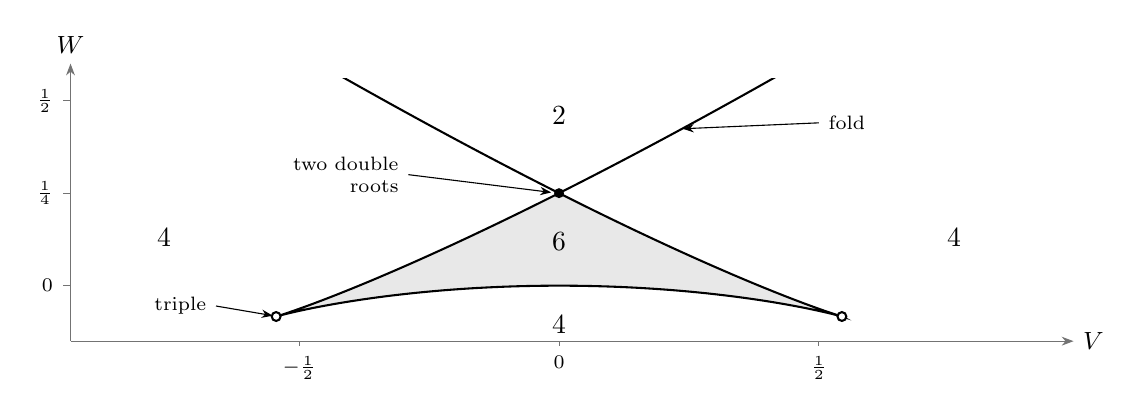
\begin{tikzpicture}[x=6.6cm,y=4.7cm,font=\small,
  boundary/.style={black,line width=.75pt},
  guide/.style={black!55,line width=.35pt},
  leader/.style={black,line width=.4pt,-{Stealth[length=1.4mm]}},
  region/.style={fill=white,inner sep=1.5pt,font=\normalsize}]
  \begin{scope}
    \clip (-.94,-.15) rectangle (.94,.56);
    % The closed central chamber has four simple quartic roots.
    \fill[black!9]
      plot[domain=-.707106781186548:.707106781186548,
        variable=\t,samples=181]
      ({2*\t-4*(\t)^3},{3*(\t)^4-(\t)^2}) -- cycle;
    \draw[boundary]
      plot[domain=-.83:.83,variable=\t,samples=301]
      ({2*\t-4*(\t)^3},{3*(\t)^4-(\t)^2});
  \end{scope}
  \draw[guide,-{Stealth[length=1.5mm]}]
    (-.94,-.15)--(.99,-.15) node[right,black] {$V$};
  \draw[guide,-{Stealth[length=1.5mm]}]
    (-.94,-.15)--(-.94,.60) node[above,black] {$W$};
  \foreach \x/\lab in {-.5/{-\tfrac12},0/0,.5/{\tfrac12}}{
    \draw[guide] (\x,-.15)--(\x,-.164);
    \node[below,font=\scriptsize] at (\x,-.164) {$\lab$};
  }
  \foreach \y/\lab in {0/0,.25/{\tfrac14},.5/{\tfrac12}}{
    \draw[guide] (-.94,\y)--(-.955,\y);
    \node[left,font=\scriptsize] at (-.955,\y) {$\lab$};
  }
  \node[region] at (0,.46) {$2$};
  \node[region,fill=black!9] at (0,.12) {$6$};
  \node[region] at (-.76,.13) {$4$};
  \node[region] at (.76,.13) {$4$};
  \node[region] at (0,-.105) {$4$};
  % Two triple-root cusp points and the two-double-root crossing.
  \draw[boundary,fill=white]
    ({-4/(3*sqrt(6))},{-1/12}) circle[radius=1.6pt];
  \draw[boundary,fill=white]
    ({4/(3*sqrt(6))},{-1/12}) circle[radius=1.6pt];
  \fill (0,.25) circle[radius=1.8pt];
  \node[anchor=east,align=right,font=\scriptsize] (dd)
    at (-.29,.30) {two double\\roots};
  \draw[leader] (dd.east)--(-.015,.252);
  \node[anchor=west,font=\scriptsize] (fold) at (.50,.44) {fold};
  \draw[leader] (fold.west)--(.238,.424);
  \node[anchor=east,font=\scriptsize] (triple) at (-.66,-.055) {triple};
  \draw[leader] (triple.east)--(-.551,-.081);
\end{tikzpicture}
\caption{A slice of the prepared quartic
$y^4+uy^2+vy+w$ at $u=-\varepsilon^2$, for any sufficiently small
$\varepsilon>0$. In the similarity coordinates
$V=v/\varepsilon^3$, $W=w/\varepsilon^4$, the multiple-root set is
$(V,W)=(2t-4t^3,3t^4-t^2)$. Region labels are the total numbers of
simple cycles, including the two simple fixed points with $q<0$.
Open circles mark triple roots; the crossing has two double roots.
This slice does not contain the quadruple-root point $u=v=w=0$.}
\label{fig:quartic-local-diagram}
\end{figure}


\FloatBarrier

\section{Realization in fields and a harvesting model}
\label{sec:sharpness}

Two constructions show that the hypotheses and the rank
condition~\eqref{eq:rank} hold. Local perturbations of an arbitrary reference
field give four independent unfolding parameters, and a two-tier harvesting
model gives them through its natural parameters. In both cases we verify the
first-return geometry and use the standard unfolding to transfer the cycle
configurations.

\subsection{Local perturbations of a given reference field}
\label{subsec:specified-field}

Fix a nonstationary reference cycle \(\mathcal C\) satisfying the geometric
hypotheses of Section~\ref{sec:passage}, with passage strengths
\(A_{1,0}=-A_{2,0}\ne0\) and closing jets
\[
 R_0(0)=0,\qquad R_0'(0)=1,\qquad
 c_0=\tfrac12R_0''(0)\ne0.
\]
The positive penetration directions agree under the regular connections,
which have no additional seam crossing. Choose a second-contact box \(U_2\)
and a smooth closing-arc flow box \(U_3\), with disjoint closures away from
the first contact and return section.
Let \(\mathcal L_{\mathcal C}(U_2,U_3)\) be the finite-dimensional
jointly smooth parameter germs through this field with seam changes
supported in \(\operatorname{int}U_2\), inactive branch fixed there,
and active difference \(h_\lambda Z_\lambda\) with smooth
\(Z_\lambda\). In \(\operatorname{int}U_3\), which stays away
from the seam, a common smooth field may be added to both branches.
All other data are fixed. The perturbations that control \((m,\delta)\)
and \((a,b)\) have disjoint supports.

\begin{proposition}[Four independent unfolding parameters]
\label{prop:specified-rank}
Every such reference field admits a four-parameter unfolding in
\(\mathcal L_{\mathcal C}(U_2,U_3)\) with
\(D_\lambda(a,b,m,\delta)\) invertible at \(\lambda=0\), which reduces to the
reference field at \(\lambda=0\). The perturbations preserve matching,
regular seams, quadratic contacts and a one-turn first-return interval.
Every finite-parameter germ in \(\mathcal L_{\mathcal C}(U_2,U_3)\) is an
admissible family after a reduction depending on the germ.
\end{proposition}

\begin{proof}
Transport the first inactive integral along the unchanged first
connector. A Morse-type normalization of the clock near the second contact
gives
\[
 X_0^-=v(t,q)\partial_t,\qquad
 X_0^+=v(t,q)\{[1+(q-t^2)\alpha(t,q)]\partial_t
                    +(q-t^2)\mu(t,q)\partial_q\},\quad v>0.
\]
For a positive smooth \(e\),
\(h_0=e(q-t^2)\) and
\(eZ_0=v(\alpha\partial_t+\mu\partial_q)\).
Choose compactly supported cutoffs \(\psi_1,\psi_2\) in \(U_2\),
equal to one on a smaller contact core, and set
\begin{equation}\label{eq:specified-contact-controls}
 h_d=h_0-de\psi_1,\qquad
 X_{\kappa,d}^+=X_0^++(h_d-h_0)Z_0
                  +\kappa h_dv\psi_2e^{-1}\partial_q,
 \qquad X_{\kappa,d}^-=X_0^-.
\end{equation}
These changes extend by zero, recover \(X_0^\pm\) at zero, and satisfy
\[
 X_{\kappa,d}^+-X_0^-
 =h_d(Z_0+\kappa v\psi_2e^{-1}\partial_q).
\]
Thus the two fields agree on the moving seam.
In the core, \(z=q-d\) gives the normalized seam \(z=t^2\) and
coefficients \(v(t,z+d),\alpha(t,z+d),\mu(t,z+d)+\kappa\).
The contact is \((0,d)\), with inactive second seam derivative
\(-2v(0,d)^2<0\) in the normalized defining function, and the
active clock stays positive. Proposition~\ref{prop:quadratic-passage}
therefore gives \(A_2(\kappa,d)=\tfrac43[\mu(0,d)+\kappa]\).
The first passage and connector are unchanged, so
\begin{equation}\label{eq:specified-strength-jacobian}
 \delta=d,\quad m=A_{1,0}+\tfrac43[\mu(0,d)+\kappa],\qquad
 D_{(\kappa,d)}(m,\delta)(0)=
 \begin{pmatrix}4/3&(4/3)\mu_q(0,0)\\0&1\end{pmatrix}.
\end{equation}
The second strength is already transported; its incoming threshold is
\(\Gamma_1^{-1}(d)\).

In \(U_3\), use the base flow time \(s\) and the second out-port
coordinate transported by that flow as \(z\). Then
\(X_0^-=\partial_s\), the entrance holonomy is \(q\mapsto z=q\),
and the remaining transition is \(R_0\). Add to both branches
\[
 Y_\eta=\chi_1(s)\chi_2(z)(\eta_0+\eta_1z)\partial_z,
 \qquad \chi_1\ge0,\qquad \int\chi_1(s)\,ds=1,
\]
with compact support and \(\chi_2=1\) on a fixed transverse interval.
Small inputs and parameters stay in that interval, so the box
holonomy and closing transition are
\[
 H_\eta(z)=e^{\eta_1}z+\eta_0\phi(\eta_1),\qquad
 \phi(w)=\int_0^1e^{wt}\,dt,\qquad R_\eta=R_0\circ H_\eta.
\]
Consequently
\begin{equation}\label{eq:specified-four-jacobian}
 D_{(\eta_0,\eta_1,\kappa,d)}(a,b,m,\delta)(0)=
 \begin{pmatrix}
 1&0&0&0\\2c_0&1&0&0\\
 0&0&4/3&(4/3)\mu_q(0,0)\\0&0&0&1
 \end{pmatrix},\qquad \det=4/3.
\end{equation}
Disjoint supports make the closing leg independent of \((\kappa,d)\).
The inverse function theorem gives the local coordinates
\((a,b,m,\delta)\).

The seam $q-t^2-d\psi_1(t,q)=0$ has $q$ derivative greater than $1/2$
for small $d$ and agrees with the old seam on a boundary collar. The
reference has a positive angular clock on a fixed tube; matching gives
common local Lipschitz bounds for the perturbed fields.
Choose cores where the cutoffs are one, ports with strict transverse margins,
and strictly inactive connecting arcs, including the cutoff collars.
Proposition~\ref{prop:quadratic-passage} gives the first entry and the
first exit in each core, with second penetration $\Gamma_1(q)-d$.
Lemma~\ref{lem:common-tube} therefore gives the one-turn return
\[
 P_\lambda(q)=R_\eta\{d+
       \Gamma_{2,\kappa,d}(\Gamma_1(q)-d)\}.
\]
For any finite-parameter germ in \(\mathcal L_{\mathcal C}(U_2,U_3)\),
matching, smooth parameter dependence and the implicit function theorem at
the contact preserve these clock, core, port and positive transverse-derivative
margins after a reduction depending on the germ.
\end{proof}

\begin{corollary}[Cyclicity in the local perturbation class]
\label{cor:specified-cyclicity}
For every reference cycle \(\mathcal C\) of
Proposition~\ref{prop:specified-rank},
\(\operatorname{Cycl}(\mathcal L_{\mathcal C}(U_2,U_3),\mathcal C)=6\) in
the sense of Definition~\ref{def:cyclicity}. The corresponding suprema over
germs contained in \(\{m=0\}\), in \(\{\delta=0\}\) and in
\(\{m=\delta=0\}\) are four, four and two. The same values hold for the class
of all admissible families through the reference field.
\end{corollary}

\begin{proof}
Each germ is admissible after its own reduction, so
Proposition~\ref{prop:common-count} gives at most six fixed points in \(I\);
the same holds for every admissible family.
Remark~\ref{rem:cycle-fixed-point} identifies the isolated fixed points
in the common interval with the nearby limit cycles. Conversely,
Proposition~\ref{prop:specified-rank} and
Proposition~\ref{prop:single-scale-six} give six simple cycles
approaching \(\mathcal C\).
Restricting the same unfolding to the three slices,
Proposition~\ref{prop:sharp-slice-attainment} attains the bounds of
Corollary~\ref{cor:four-slices}. Since the families of
Proposition~\ref{prop:specified-rank} are admissible, the same values hold for
the class of all admissible families; this proves part~3 of
Theorem~\ref{thm:six-main}.
\end{proof}

\subsection{A two-tier escapement-harvesting model}
\label{sec:harvesting}

This model shows that the hypotheses and the rank condition hold for the
natural parameters of an ecological family. Continuous threshold harvesting,
which switches harvest on continuously above a population threshold, is
studied in~\cite{leardrebaza2011,rebaza2012}. The policy of Bohn, Rebaza and
Speer~\cite{bohn2011} stops prey harvest below a lower threshold, increases it
linearly between two thresholds and caps it above the upper one; Onana Ndzana
et al.~\cite{onana2019} use it in a delayed Leslie--Gower model with prey
refuge. We intensify harvest above the upper threshold, using the normalized
smooth
predator-harvesting core of Huang, Gong and Ruan
\cite[equation~(9) and Theorem~3.6]{huang2013}:
\begin{equation}\label{eq:harvesting:model}
 \dot x=x(1-x-y)-u(x-L)_+-v(x-U)_+,\qquad
 \dot y=y\left(d-\beta\frac yx\right)-h.
\end{equation}
Here \(x,y>0\) are prey and predator densities,
\(\beta,d,h,u,v>0\), and \(0<L<U<1\).
The predator parameters \(d,\beta,h\) describe growth, density limitation
relative to prey abundance, and constant-yield harvest.
The marginal prey efforts are \(0,u,u+v\). We work in a compact
subset of the positive quadrant. The middle smooth extension is
\begin{equation}\label{eq:harvesting:middle}
 F_c=x(1-x-y)-u(x-L),\qquad
 G=y(d-\beta y/x)-h,\qquad X_c=(F_c,G),
\end{equation}
and the exterior extensions are
\[
 X_\ell=(x(1-x-y),G),\qquad X_r=(F_c-v(x-U),G).
\]
The adjacent extensions agree on the whole seams:
\(X_\ell=X_c\) on \(x=L\) and \(X_c=X_r\) on \(x=U\).
The middle extension is
inactive at both contacts, with active sides outside \(L\le x\le U\).
The branches are analytic for \(x>0\) and the field is
locally Lipschitz.

\begin{theorem}[Natural harvesting realization]
\label{thm:harvesting-realization}
There exists \(\rho_0>0\) such that, for every fixed radius
\(0<\rho<\rho_0\) in the smooth-core fold construction of
Appendix~\ref{app:harvesting-fold}, there exists \(u_0(\rho)>0\) with the following
property. For every fixed \(0<u<u_0(\rho)\) there are positive parameters
\(\beta,d,h,v\) and thresholds \(0<L<U<1\), depending on \(\rho\) and \(u\),
for which \eqref{eq:harvesting:model} has an embedded semistable periodic
orbit \(\mathcal C\) with exactly two quadratic contacts, at its minimum and
maximum prey densities. In one transported return coordinate the contact
levels agree and
\[
 A_1=A_0=-A_2\ne0,\qquad
 R(0)=0,\qquad R'(0)=1,\qquad c_0=\tfrac12R''(0)<0.
\]
The map \(\lambda\mapsto(a,b,m,\delta)\) has rank four in the natural
family \(\lambda=(\beta,d,h,u,v,L,U)\). The cyclicity of \(\mathcal C\) in
this family is six, and the corresponding values on \(m=0\), on
\(\delta=0\) and on their intersection are four, four and two. The
conclusions of Theorems~\ref{thm:main-saturation-summary}
and~\ref{thm:actual-quartic-summary} hold for the standard unfolding of this
family (Corollary~\ref{cor:realization-transfer}).
\end{theorem}

We construct a smooth cyclic fold, fit the thresholds to its prey
extrema, and cancel the passage strengths with a positive effort
ratio. The directions \((\nu,L,v,U)\), with \(\beta,u\) fixed,
then give the standard unfolding.

\subsection{Threshold fitting, cancellation and closing curvature}

Appendix~\ref{app:harvesting-fold} constructs cyclic folds of
the smooth core, for every sufficiently small fixed radius \(\rho>0\).
The fold is embedded and nonstationary, lies in the positive quadrant,
and has exactly one nondegenerate prey minimum and maximum. In radial
coordinates its displacement satisfies
\eqref{eq:harvesting:fold-data}, with \(\ell<0\), and the
\((\beta,\nu)\) Jacobian of \((D,D_r)\) is invertible.
These strict properties allow the thresholds and positive efforts to be
fitted to a fixed fold.

For positive \(u\), use
\begin{equation}\label{eq:harvesting:perturbed-chart}
 y_e=\tfrac45-u(1-5L),\qquad
 d=8\beta+\tfrac15+\nu,\qquad h=y_e(d-5\beta y_e).
\end{equation}
The middle field vanishes at \((1/5,y_e)\). At \(u=0\) the chart
reduces to \eqref{eq:harvesting:core-chart} and is independent of
\(L\). Fix a positive fold radius in
\eqref{eq:harvesting:fold-data}. The invertible \((\beta,\nu)\)
Jacobian of \((D,D_r)\) continues a fold \(\mathcal C(u,L)\)
for small \(u,L-L_0\), where \(L_0\) is the unperturbed prey
minimum. Its curvature and two nondegenerate extrema persist.
For its minimum \(x_{\min}(u,L)\),
\(\partial_Lx_{\min}(0,L_0)=0\), so
\begin{equation}\label{eq:harvesting:threshold-fit}
 L=x_{\min}(u,L),\qquad U=\max_x\mathcal C(u,L(u))
\end{equation}
has a unique local smooth solution with \(0<L(u)<U(u)<1\).
After reducing \(u\), all parameters in
\eqref{eq:harvesting:perturbed-chart} remain positive. The fitted
orbit stays in the closed middle strip, touching its boundary only
at the extrema, and is an orbit of \eqref{eq:harvesting:model} for every \(v\). There
\(F_c=0\), \(F_{c,y}=-x\), and nonstationarity gives \(G\ne0\),
so
\begin{equation}\label{eq:harvesting:quadratic-contact}
 \ddot x=F_{c,y}G=-xG\ne0.
\end{equation}

Figure~\ref{fig:harvesting-orbit} illustrates this fitted threshold geometry.
For each of two fixed parameter tuples, Online Resource~3 proves by interval
arithmetic the existence of at least six distinct simple periodic orbits of
\eqref{eq:harvesting:model}. Theorem~\ref{thm:harvesting-realization} is analytic and does not depend on
these certificates.
\begin{figure}[tb]
 \centering
 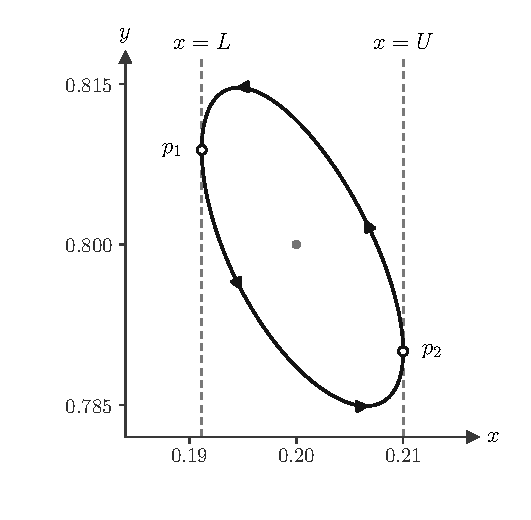
\includegraphics[width=90mm]{figures/harvesting-orbit.pdf}
 \caption{Numerical illustration of the fitted threshold geometry of
 \eqref{eq:harvesting:model}. With \(u=10^{-6}\) and \(U=0.21\)
 prescribed, the resulting parameter values are
 \(\beta\simeq0.031443254\), \(d\simeq0.451546877\),
 \(h\simeq0.260619080\), and \(L\simeq0.191154841\).
 The middle orbit touches the vertical thresholds \(x=L\) and \(x=U\)
 at its prey extrema. Open circles mark the contacts \(p_1,p_2\),
 arrows show increasing time, and the dot marks the middle
 equilibrium. Theorem~\ref{thm:harvesting-realization} proves the existence
 of such reference cycles and their six-cycle unfoldings.}
 \label{fig:harvesting-orbit}
\end{figure}

Positive penetration is outward, into \(x<L\) or \(x>U\).
At \(p_i=(x_i,y_i)\), write \(G_i=G(p_i)\).
Equation~\eqref{eq:harvesting:quadratic-contact} gives \(G_1<0<G_2\), so
\(y=y_i\) are transverse sections. In the coordinates \(z_1=L-x\),
\(z_2=x-U\), their inactive transitions along the forward arcs satisfy
\[
 S_1'(0)=-\frac{G_1}{G_2}
       \exp\!\int_{p_1}^{p_2}\operatorname{div}X_c\,dt>0,
 \qquad
 S_2'(0)=-\frac{G_2}{G_1}
       \exp\!\int_{p_2}^{p_1}\operatorname{div}X_c\,dt>0.
\]
Positive penetration normalizations preserve these signs and, on a common
smaller domain, give positive derivative margins.
Transport one inactive first integral \(I\) from the first box through
the connector to the second, with outward direction positive. These are
local first-integral charts joined along the connecting tube. At
\(p_i\), put \(\sigma_1=-1\), \(\sigma_2=1\),
\(s_i=I_x(p_i)\). Then \(I_y(p_i)=0\) and
\(\sgn s_i=\sigma_i\). A Morse-type normalization of the clock for
\(\mathfrak h_i=\sigma_i(x-x_i)\), preserving \(I\), gives
\begin{equation}\label{eq:harvesting:clock}
 \mathfrak h_i=e_i(t,I)(I-t^2),\qquad
 e_i(0,0)=\frac{\sigma_i}{s_i}>0,\qquad
 \dot t(0,0)=\omega_i
 =\sqrt{-s_iF_{c,y}(p_i)G(p_i)/2}>0.
\end{equation}
These clocks differ from the core frequency \(\omega\). For active
difference \(\mathfrak h_iZ_i\), the normalized transverse coefficient is
\[
 \mu_i(0,0)
 =\frac{e_i(0,0)}{\omega_i}dI(Z_i)
 =\frac{\sigma_i(Z_i)_x}{\omega_i}.
\]
Here \(Z_1=-u\partial_x\), \(Z_2=-v\partial_x\); thus
\eqref{eq:passage:strength-jet} gives
\begin{equation}\label{eq:harvesting:strengths}
 A_1=K_1u=\frac{4u}{3\omega_1}>0,\qquad
 A_2=-K_2v=-\frac{4v}{3\omega_2}<0.
\end{equation}
The opposing passage signs come from the opposite outward directions at
the two thresholds; both harvesting efforts are positive.
The inactive clocks and transport are independent of \(v\), so
the exact positive ratio
\begin{equation}\label{eq:harvesting:effort-relation}
 v=u\frac{K_1}{K_2}=u\frac{\omega_2}{\omega_1}
\end{equation}
cancels the strengths in the same transported coordinate.
Both contacts lie on one inactive orbit, so their levels agree.
Their passage derivatives equal one at the touch and the middle fold
has multiplier one. Lemma~\ref{lem:passage:finite-inverse} gives
\(Q(q)=q+q_+^{5/2}\mathcal L(\sqrt{q_+})\), with no terms of order
\(q^{3/2}\) or \(q^2\). The regular map \(R\) is the inactive monodromy.

The closing curvature \(c_0\) is negative in the outward-positive coordinate. First
set \(u=0\) and fix the cyclic-fold parameters at a small radius
\(\rho\). Vary the initial radial coordinate \(r\) with these
parameters fixed. Smooth finite-time normal-form flow has prey component
\[
 x(r,\theta)=\tfrac15+rp(\theta)+O(r^2+\rho^2r),
\]
where \(p\) is a nonzero first harmonic and the \(r\)-derivative
of the remainder is \(O(r+\rho^2)\). Its unique nearby prey minimum
\(M(r)\) satisfies \(M'(\rho)=-\gamma+O(\rho)<0\), \(\gamma>0\).
The minimum locus \(F_c=0\) is transverse, since its derivative
along the orbit is \(\ddot x\ne0\). If \(H(r)\) is the
transported inactive integral there, \(I_y=0\), \(I_x<0\) give
\(H'(\rho)=I_xM'(\rho)>0\). For the radial core return \(P_c\)
at these fixed parameters,
\(R=H\circ P_c\circ H^{-1}\). At the fixed point, where \(R'=1\),
\[
 R''(0)=\frac{P_c''(\rho)}{H'(\rho)}<0
\]
by \eqref{eq:harvesting:fold-data} and \(\ell<0\).
Continuation to fitted small positive \(u\) preserves this strict
sign and \(H'>0\). The cancelling composition has zero quadratic
defect, so \(c_0<0\) for the reference cycle as well.

\subsection{Rank condition and first return}

At the fitted orbit we now show that the four return-map controls can be
varied independently and that nearby orbits keep the first-return structure.

Use \((\nu,L,v,U)\) in \eqref{eq:harvesting:perturbed-chart}, with
\(\beta,u\) fixed. Choose the first incoming coordinate from the
middle extension and lower seam only. The regular monodromy \(R\)
is independent of \(v,U\): changes of the upper ports alter the
intermediate inactive holonomies but preserve their middle-return
composition. The threshold separation \(\delta\) is independent of
\(v\). At the upper tangency \(F_c(U,y_2(U))=0\) and \(I_y=0\),
so
\begin{equation}\label{eq:harvesting:upper-rank}
 \delta_U=I_x(p_2)\ne0,\qquad m_v=-K_2\ne0.
\end{equation}
Hence
\begin{equation}\label{eq:harvesting:rank-matrix}
 D_{(\nu,L,v,U)}(a,b,m,\delta)=
 \begin{pmatrix}
 a_\nu&a_L&0&0\\ b_\nu&b_L&0&0\\
 *&*&-K_2&*\\ *&*&0&\delta_U
 \end{pmatrix}.
\end{equation}
For the upper-left minor first set \(u=0\) at the fixed core fold.
The lower tangency is \(p_1(L)=(L,1-L)\); its level in an unchanged
core transverse coordinate has derivative
\begin{equation}\label{eq:harvesting:lower-level}
 \zeta_L=dI(p_1'(L))=I_x(p_1)\ne0.
\end{equation}
Choose this coordinate to agree with the incoming one at the base,
and centre the contact by \(T_L(\zeta(L))=0\). Then
\(R_L=T_L\circ P_c\circ T_L^{-1}\). Since at the fold
\(P_c(\zeta)=\zeta\) and \(P_c'(\zeta)=1\),
\begin{equation}\label{eq:harvesting:lower-rank}
 a_L=0,\qquad b_L=P_c''(\zeta)\zeta_L
                   =2c_0\zeta_L\ne0.
\end{equation}
At \(u=0\), the core return \(P_c\) is independent of \(L\), so the
\(L\)-dependence of \(R_L\) comes only from the moving section. Because
the base coordinates agree and \(D_r=0\), contact motion leaves the
offset derivative in \(\nu\) unchanged;
\eqref{eq:harvesting:scaled-return} gives \(a_\nu\ne0\). Moving-coordinate
terms in \(b_\nu\) do not enter the minor since \(a_L=0\). Thus the minor
is \(a_\nu\,2c_0\zeta_L\ne0\); another transverse scaling changes it
only by a nonzero factor. These objects extend smoothly to
\(u=0\), so at each fixed radius the minor persists for small
positive \(u\), with fitted thresholds and
\eqref{eq:harvesting:effort-relation}. All couplings remain in
\eqref{eq:harvesting:rank-matrix}, whose determinant is the minor
times \((-K_2)\delta_U\ne0\). The chart directions embed in
\((\beta,d,h,u,v,L,U)\), proving~\eqref{eq:rank} in the natural
parameters.

The fitted cycle is compact, embedded and nonstationary. On a fixed tube,
the vertical seams stay regular and the matched model has common local
Lipschitz bounds. The positive angular clock, transverse ports, positive
transverse-derivative margins and strictly inactive connectors persist under
small parameter changes. In each core,
\eqref{eq:harvesting:clock} and the smooth active difference satisfy the
passage hypotheses, including first entry and first exit.
Lemma~\ref{lem:common-tube} gives the chronological first return on one
common interval. Thus each constructed reference satisfies the geometric
first-return hypotheses as well as the rank condition.

\subsection{Transfer to the natural parameters}

\begin{corollary}[Main results in the constructed families]
\label{cor:realization-transfer}
For each reference constructed above, with its standard unfolding and
interval \(I\), the bounds and attainment of Theorem~\ref{thm:six-main} hold.
In the sign case $A_1(\lambda_0)=B>0$, $c_0=-C<0$, which includes every
harvesting reference, the conclusions of
Theorem~\ref{thm:main-saturation-summary}, Theorem~\ref{thm:actual-quartic}
and Proposition~\ref{quartic:strata} hold for the same unfolding on \(I\).
In the harvesting family all parameters remain positive and $0<L<U<1$.
\end{corollary}

\begin{proof}
The Jacobians \eqref{eq:specified-four-jacobian} and
\eqref{eq:harvesting:rank-matrix}, together with
Lemma~\ref{lem:common-tube}, give the standard unfolding and common interval.
Fix this unfolding before choosing the scale: every compact set of rescaled
controls lies in the domain of its inverse \(\Lambda\) at sufficiently small
scale. In the harvesting family the inverse maps \((a,b,m,\delta)\) to
\((\nu,L,v,U)\), with \(\beta,u\) fixed, preserving positivity and
$0<L<U<1$. Apply Theorems~\ref{thm:six-main}
and~\ref{thm:main-saturation-summary}. In the stated sign case,
Lemma~\ref{mainloc:all-roots} localizes all roots in \(I\): two simple
negative roots and a positive cluster beyond both thresholds.
Theorem~\ref{thm:actual-quartic} and Proposition~\ref{quartic:strata}
give its preparation and strata. Remark~\ref{rem:cycle-fixed-point}
identifies the isolated fixed points with cycles, completing
Theorem~\ref{thm:harvesting-realization}.
\end{proof}

\section{Concluding remarks}\label{sec:concluding}

A cancellation that makes the reference return map $C^2$ need not make its
unfoldings jointly $C^2$. The aligned cancelling slice has cyclicity two,
whereas a full-rank unfolding of all four return-map controls attains six
limit cycles. Several questions remain open.
\begin{enumerate}
\item Theorem~\ref{thm:main-saturation-summary} describes the limit of the
saturation domains. Apart from the fourfold point of
Theorem~\ref{thm:actual-quartic-summary} and the corner $S_4\to0$ treated in
Online Resource~1, the number of limit cycles at positive scale for parameters
near boundary points of $\mathcal K_4$ is not determined here.
\item Parts~2 and~3 of Theorem~\ref{thm:main-saturation-summary} and
Theorem~\ref{thm:actual-quartic-summary} are stated in the sign case
$A_1(\lambda_0)>0$, $c_0<0$. The remaining sign cases are not treated here.
\item A periodic orbit tangent to two switching lines of a discontinuous
system with sliding is studied in~\cite{roitenberg2025}. The effect of
cancelling leading terms in the presence of sliding is open.
\item The contacts here are quadratic. For tangencies of higher order the
corrections have other exponents, and the interaction between cancellation
and moving thresholds remains to be analysed.
\end{enumerate}

\appendix
\section{Smooth-core folds and finite focus equations}
\label{app:harvesting-fold}

Threshold fitting uses a smooth-core cyclic fold with negative return
curvature and a nonsingular two-parameter fold equation. We derive these
inputs from finite focus equations and control the one-turn remainder
with the required state and parameter derivatives.

\subsection{The core chart and its focus coefficients}

At \(u=0\), use the equilibrium-preserving chart
\begin{equation}\label{eq:harvesting:core-chart}
 d=8\beta+\tfrac15+\nu,\qquad
 h=\tfrac{16}{5}\beta+\tfrac4{25}+\tfrac45\nu.
\end{equation}
The equilibrium is \((1/5,4/5)\), with
\[
 J=\begin{pmatrix}-1/5&-1/5\\16\beta&1/5+\nu\end{pmatrix},
 \qquad \operatorname{tr}J=\nu,\qquad
 \det J=\frac{80\beta-1-5\nu}{25}.
\]
The multiplicity-two weak focus of
\cite[Theorem~3.6]{huang2013} occurs at
\begin{equation}\label{eq:harvesting:bautin-point}
 \beta_0=\frac{\sqrt{51}-4}{100},\qquad
 d_0=\frac{-3+2\sqrt{51}}{25},\qquad
 h_0=\frac{4(1+\sqrt{51})}{125},\qquad \nu=0.
\end{equation}
The finite homogeneous equations below construct \(V=\mathcal R^2/2+\bigO(\mathcal R^3)\) in rotation
coordinates of radius \(\mathcal R\), and give
\begin{equation}\label{eq:harvesting:focus-data}
 k_4=\ell_1(\beta)
 =\frac{25\beta(2000\beta^2+160\beta-7)}{4(80\beta-1)},
 \qquad k_6\big|_{\beta=\beta_0}
 =-\frac{155}{48}-\frac{235\sqrt{51}}{576}<0.
\end{equation}
Thus \(\ell_1(\beta_0)=0\) and
\(\ell_1'(\beta_0)=17/2+4\sqrt{51}>0\). At the focus,
\(\dot V=k_6\mathcal R^6+\bigO(\mathcal R^7)\), so
\(\sqrt{2V}\) has nonzero negative quintic drift. The angular
velocity tends to
\(\omega_0=\sqrt{(-21+4\sqrt{51})/125}>0\); positive radial
scaling and angular clock therefore give \(\ell<0\) below.
The conjugate eigenvalues of \(J\) have real part \(\nu/2\), and
\((\nu,\beta)\mapsto(\nu/2,\ell_1(\beta))\) has rank two at
\((0,\beta_0)\).

At \(u=\nu=0\), put
\(\omega^2=(80\beta-1)/25\), \(X=x-1/5\), and
\(Z=(x-1/5+y-4/5)/(5\omega)\). Direct substitution gives
\begin{equation}\label{eq:harvesting:rotation}
 \dot X=-\omega Z+\Phi,\qquad
 \dot Z=\omega X+\Psi,\qquad \Phi=-5\omega XZ,
\end{equation}
where
\[
 \Psi=-\frac{
 80\omega X^2Z+(125\omega^2+5)X^2
 +(6\omega-250\omega^3)XZ
 +(125\omega^4+5\omega^2)Z^2}
 {16\omega(5X+1)}.
\]
Expand \((1+5X)^{-1}\) through the degrees needed below and denote
homogeneous terms by subscripts. For
\(\mathcal R^2=X^2+Z^2\), seek
\(V=\mathcal R^2/2+V_3+\cdots+V_6\). The equations are
\begin{equation}\label{eq:harvesting:homological}
 \mathcal L V_n=k_n\mathcal R^n-H_n,\qquad
 \mathcal L=\omega(-Z\partial_X+X\partial_Z),\qquad
 H_n=\sum_{j=2}^{n-1}
 \bigl(\partial_XV_j\,\Phi_{n-j+1}
       +\partial_ZV_j\,\Psi_{n-j+1}\bigr).
\end{equation}
Here \(V_2=\mathcal R^2/2\). On homogeneous polynomials of odd degree
\(n\), \(\mathcal L\) is invertible and \(k_n=0\); for even \(n\), take
the radial obstruction
\[
 k_n=\frac1{2\pi}\int_0^{2\pi}
 H_n(\cos\theta,\sin\theta)\,d\theta
\]
and set the \(X^n\) coefficient of \(V_n\) to zero to fix the radial
kernel. Solving \eqref{eq:harvesting:homological} successively in the
monomial basis for $n=3,4,5,6$ gives
$k_3=k_5=0$ and the coefficients~\eqref{eq:harvesting:focus-data}.
A program in Online Resource~2, also included with the source files,
reconstructs the rotated field and checks every coefficient residual of these
finite equations in exact arithmetic.

\subsection{Normal form and cyclic folds}

The focus coefficients supply the generalized Hopf unfolding. Its
weighted return turns the limiting fold into a periodic orbit with the
geometry required at the thresholds.

Take the finite normal form through degree
seven in a parameter-dependent complex coordinate. Its nonresonant
divisors stay bounded away from zero near the positive frequency
\(\omega_0\); hence the transformations and their required parameter
derivatives are smooth. The retained resonant degrees are one,
three, five and seven. Division by the positive angular speed and
normalization of one turn give smooth coefficients \(\eta_1,\eta_2\)
for the first two radial terms, with invertible
\((\nu,\beta)\mapsto(\eta_1,\eta_2)\) Jacobian. The fifth-degree
coefficient equals \(\ell\ne0\) at the focus. For the generalized Hopf normal
form see~\cite{kuznetsov2023}; its coefficients for ordinary and delay
equations are also derived by N.~A.~M.~Delmeire, M.~M.~Bosschaert and
Yu.~A.~Kuznetsov (preprint, 2025,
\href{https://arxiv.org/abs/2507.18469v1}{arXiv:2507.18469v1}).
Normalize the angular clock to one turn and put
\(r=\rho z\), \(\eta_1=\rho^4s_1\), \(\eta_2=\rho^2s_2\).
Then
\begin{equation}\label{eq:harvesting:weighted-flow}
 \frac{dz}{d\theta}
 =\rho^4(s_1z+s_2z^3+\ell z^5)+\bigO(\rho^6),\qquad \ell<0.
\end{equation}
On a fixed positive \(z\)-interval about one, the bound holds after
two \(z\) derivatives and one derivative in \((s_1,s_2)\), including
mixed derivatives. The quintic coefficient varies by \(\bigO(\rho^2)\),
giving \(\bigO(\rho^6)\) in the scaled equation, as does the retained
seventh-degree term; the smooth degree-eight field remainder gives
\(\bigO(\rho^7)\). Taylor remainders preserve these state bounds,
and scaled parameter differentiation introduces a factor \(\rho^4\)
or \(\rho^2\). The angular speed retains a positive uniform margin.
Integration over one turn and smooth finite-time flow dependence give
the smooth-core displacement
\begin{equation}\label{eq:harvesting:scaled-return}
 \rho^{-5}D(\rho z;\rho^4s_1,\rho^2s_2)
 =s_1z+s_2z^3+\ell z^5+\smallO(1)
\end{equation}
in the same norms, including angle-dependent remainders.
At \(z=1\), the limiting fold equations
\(s_1+s_2+\ell=0\), \(s_1+3s_2+5\ell=0\) have parameter
determinant two. Hence for every sufficiently small positive \(\rho\)
the implicit function theorem gives a cyclic fold with
\begin{equation}\label{eq:harvesting:fold-data}
 \eta_1=\ell\rho^4+\smallO(\rho^4),\qquad
 \eta_2=-2\ell\rho^2+\smallO(\rho^2),\qquad
 D_{rr}(\rho)=8\ell\rho^3+\smallO(\rho^3)\ne0.
\end{equation}
The \((D,D_r)\) parameter determinant is a nonzero
coordinate factor times \(2\rho^3+\smallO(\rho^3)\). Moreover,
\(\partial_\nu\eta_1\ne0\) at the generalized Hopf point and
\[
 \partial_\nu D(\rho)
 =\rho\partial_\nu\eta_1+\smallO(\rho)\ne0.
\]
These margins are strict at each fixed positive radius.
After division by \(\rho\), the fold orbit is \(C^2\)-close to a
Hopf ellipse. Its prey derivative is close to a nonzero sinusoid,
with strict sign away from two simple zeros and strict monotonicity
near them. Thus the orbit is embedded and nonstationary, has exactly
one nondegenerate prey minimum and maximum, and lies in a compact
subset of \(x,y>0\).
This is the fold used to fit the lower and upper thresholds in the
harvesting model.

\section*{Acknowledgments and AI tool disclosure}

OpenAI’s ChatGPT and Codex were used during the development and preparation of this work. These tools assisted with exploring proof strategies, developing and checking mathematical arguments, preparing verification scripts, and revising the exposition and LaTeX source. They were also used to help identify relevant literature and potential gaps in intermediate drafts. The author is responsible for the mathematical claims, references, and final presentation of the paper.

\section*{Statements and Declarations}

\paragraph{Funding.}
The author received no funding for this work.

\paragraph{Competing interests.}
The author has no competing interests to declare.

\paragraph{Author contributions.}
Haibo Lu was responsible for the research design, mathematical analysis,
computational verification, and writing and revision of the manuscript.

\paragraph{Data and code availability.}
The editable manuscript source, retained figures, and finite checking scripts
accompany this paper. Online Resource~1 contains the mathematical
supplement on secondary saturation and cusp geometry. Online Resource~2
reproduces the finite exact focus computation described in
Appendix~\ref{app:harvesting-fold}, and contains further independent symbolic
checks with their inputs and recorded outputs, together with a floating-point
diagnostic of the harvesting model. Online
Resource~3 contains computer-assisted proofs that, at each of two fixed parameter
tuples, the harvesting model has at least six distinct simple periodic orbits,
with exact inputs, recorded enclosures, dependencies and
reproduction instructions. The analytic results are proved in the text; the
computational files provide independent checks and fixed-parameter
examples.

\paragraph{Supplementary material captions.}
\emph{Online Resource~1 (ESM\_1.pdf).} Secondary Saturation and Cusp Geometry
at Cancelling Double Grazing: secondary-scale domains, realization with
positive closing offset and the secondary cusp.
\emph{Online Resource~2 (ESM\_2.zip).} Independent symbolic verification:
finite focus and passage calculations, control-rank determinant identities
under the stated analytic hypotheses, and quartic algebra, with the supplied
inputs, recorded outputs and a floating-point harvesting diagnostic.
\emph{Online Resource~3 (ESM\_3.zip).} Independent interval return
certificates for at least six simple cycles at each of two fixed
harvesting parameter tuples, with input validation and recorded enclosures.

\begin{thebibliography}{99}
\setlength{\itemsep}{1pt}

\bibitem{bohn2011}
J.~Bohn, J.~Rebaza and K.~Speer,
Continuous Threshold Prey Harvesting in Predator-Prey Models,
\emph{International Journal of Mathematical and Computational Sciences}
\textbf{5} (2011), no.~7, 996--1003.
\href{https://publications.waset.org/11256/continuous-threshold-prey-harvesting-in-predator-prey-models}{publications.waset.org/11256}.

\bibitem{bonetseara2016}
C.~Bonet-Rev\'es and T.~M-Seara,
Regularization of sliding global bifurcations derived from the local fold
singularity of Filippov systems,
\emph{Discrete and Continuous Dynamical Systems}
\textbf{36} (2016), 3545--3601.
\url{https://doi.org/10.3934/dcds.2016.36.3545}.

\bibitem{bonetseara2022}
C.~Bonet-Rev\'es and T.~M-Seara,
Two regularizations of the grazing-sliding bifurcation giving non
equivalent dynamics,
\emph{Journal of Differential Equations}
\textbf{332} (2022), 219--277.
\url{https://doi.org/10.1016/j.jde.2022.05.028}.

\bibitem{colombodercole2010}
A.~Colombo and F.~Dercole,
Discontinuity Induced Bifurcations of Nonhyperbolic Cycles in
Nonsmooth Systems,
\emph{SIAM Journal on Applied Dynamical Systems}
\textbf{9} (2010), 62--83.
\url{https://doi.org/10.1137/080732377}.

\bibitem{colombo2012}
A.~Colombo, M.~di Bernardo, S.~J.~Hogan and M.~R.~Jeffrey,
Bifurcations of piecewise smooth flows: perspectives, methodologies and open
problems,
\emph{Physica D} \textbf{241} (2012), 1845--1860.
\url{https://doi.org/10.1016/j.physd.2011.09.017}.

\bibitem{dibbc2001}
M.~di Bernardo, C.~J.~Budd and A.~R.~Champneys,
Normal form maps for grazing bifurcations in \(n\)-dimensional
piecewise-smooth dynamical systems,
\emph{Physica D} \textbf{160} (2001), 222--254.
\url{https://doi.org/10.1016/S0167-2789(01)00349-9}.

\bibitem{dibernardo2008}
M.~di Bernardo, C.~J.~Budd, A.~R.~Champneys and P.~Kowalczyk,
\emph{Piecewise-smooth Dynamical Systems: Theory and Applications},
Applied Mathematical Sciences \textbf{163}, Springer, London, 2008.
\url{https://doi.org/10.1007/978-1-84628-708-4}.

\bibitem{dumortierroussarie2008}
F.~Dumortier and R.~Roussarie,
Multi-layer canard cycles and translated power functions,
\emph{Journal of Differential Equations} \textbf{244} (2008), 1329--1358.
\url{https://doi.org/10.1016/j.jde.2007.08.013}.
Corrigendum, \textbf{245} (2008), 1995.
\url{https://doi.org/10.1016/j.jde.2008.07.018}.

\bibitem{freire1998}
E.~Freire, E.~Ponce, F.~Rodrigo and F.~Torres,
Bifurcation sets of continuous piecewise linear systems with two zones,
\emph{International Journal of Bifurcation and Chaos}
\textbf{8} (1998), 2073--2097.
\url{https://doi.org/10.1142/S0218127498001728}.

\bibitem{golubitsky1973}
M.~Golubitsky and V.~Guillemin,
\emph{Stable Mappings and Their Singularities},
Graduate Texts in Mathematics \textbf{14}, Springer, New York, 1973.
\url{https://doi.org/10.1007/978-1-4615-7904-5}.

\bibitem{guardia2011}
M.~Guardia, T.~M.~Seara and M.~A.~Teixeira,
Generic bifurcations of low codimension of planar Filippov systems,
\emph{Journal of Differential Equations} \textbf{250} (2011), 1967--2023.
\url{https://doi.org/10.1016/j.jde.2010.11.016}.

\bibitem{huang2013}
J.~Huang, Y.~Gong and S.~Ruan,
Bifurcation analysis in a predator-prey model with constant-yield
predator harvesting,
\emph{Discrete and Continuous Dynamical Systems--B}
\textbf{18} (2013), 2101--2121.
\url{https://doi.org/10.3934/dcdsb.2013.18.2101}.

\bibitem{kowalczyk2006}
P.~Kowalczyk, M.~di Bernardo, A.~R.~Champneys, S.~J.~Hogan,
M.~E.~Homer, P.~T.~Piiroinen, Y.~A.~Kuznetsov and A.~B.~Nordmark,
Two-parameter discontinuity-induced bifurcations of limit cycles:
classification and open problems,
\emph{International Journal of Bifurcation and Chaos}
\textbf{16} (2006), 601--629.
\url{https://doi.org/10.1142/S0218127406015015}.

\bibitem{kuznetsov2023}
Yu.~A.~Kuznetsov,
\emph{Elements of Applied Bifurcation Theory}, 4th edn.,
Applied Mathematical Sciences \textbf{112}, Springer, Cham, 2023.
\url{https://doi.org/10.1007/978-3-031-22007-4}.

\bibitem{kuznetsov2003}
Yu.~A.~Kuznetsov, S.~Rinaldi and A.~Gragnani,
One-parameter bifurcations in planar Filippov systems,
\emph{International Journal of Bifurcation and Chaos}
\textbf{13} (2003), 2157--2188.
\url{https://doi.org/10.1142/S0218127403007874}.

\bibitem{leardrebaza2011}
B.~Leard and J.~Rebaza,
Analysis of predator--prey models with continuous threshold harvesting,
\emph{Applied Mathematics and Computation} \textbf{217} (2011), no.~12,
5265--5278.
\url{https://doi.org/10.1016/j.amc.2010.11.050}.

\bibitem{liweitanxi2014}
Q.~Li, L.~Wei, J.~Tan and J.~Xi,
Double Grazing Periodic Motions and Bifurcations in a Vibroimpact System
with Bilateral Stops,
\emph{Abstract and Applied Analysis}
\textbf{2014} (2014), article 642589, 9 pages.
\url{https://doi.org/10.1155/2014/642589}.

\bibitem{lilimeng2021}
S.~Li, Q.~Li and Z.~Meng,
Dynamic Behaviors of a Two-Degree-of-Freedom Impact Oscillator
with Two-Sided Constraints,
\emph{Shock and Vibration}
\textbf{2021} (2021), no.~1, article 8854115, 14 pages.
\url{https://doi.org/10.1155/2021/8854115}.

\bibitem{liuyue2023}
R.~Liu and Y.~Yue,
Composite Poincar\'e mapping of double grazing in non-smooth
dynamical systems: bifurcations and insights,
\emph{Acta Mechanica} \textbf{234} (2023), 4573--4587.
\url{https://doi.org/10.1007/s00707-023-03602-6}.

\bibitem{miao2023}
P.~Miao, D.~Li, S.~Yin, J.~Xie, C.~Grebogi and Y.~Yue,
Double grazing bifurcations of the non-smooth railway wheelset systems,
\emph{Nonlinear Dynamics} \textbf{111} (2023), 2093--2110.
\url{https://doi.org/10.1007/s11071-022-07926-1}.

\bibitem{nordmark1991}
A.~B.~Nordmark,
Non-periodic motion caused by grazing incidence in an impact oscillator,
\emph{Journal of Sound and Vibration} \textbf{145} (1991), no.~2, 279--297.
\url{https://doi.org/10.1016/0022-460X(91)90592-8}.

\bibitem{nordmark2002}
A.~B.~Nordmark,
Discontinuity mappings for vector fields with higher order continuity,
\emph{Dynamical Systems} \textbf{17} (2002), 359--376.
\url{https://doi.org/10.1080/1468936021000041645}.

\bibitem{novaessilva2021}
D.~D.~Novaes and L.~A.~Silva,
Lyapunov coefficients for monodromic tangential singularities in
Filippov vector fields,
\emph{Journal of Differential Equations} \textbf{300} (2021), 565--596.
\url{https://doi.org/10.1016/j.jde.2021.08.008}.

\bibitem{novaessilva2025}
D.~D.~Novaes and L.~A.~Silva,
Unveiling the cyclicity of monodromic tangential singularities:
insights beyond the pseudo-Hopf bifurcation,
\emph{SIAM Journal on Applied Dynamical Systems}
\textbf{24} (2025), 165--186.
\url{https://doi.org/10.1137/24M1668329}.

\bibitem{novaesteixeirazeli2018}
D.~D.~Novaes, M.~A.~Teixeira and I.~O.~Zeli,
The generic unfolding of a codimension-two connection to a two-fold
singularity of planar Filippov systems,
\emph{Nonlinearity} \textbf{31} (2018), 2083--2104.
\url{https://doi.org/10.1088/1361-6544/aaaaf7}.

\bibitem{ofarrell2008}
A.~G.~O'Farrell,
Composition of involutive power series, and reversible series,
\emph{Computational Methods and Function Theory}
\textbf{8} (2008), 173--193.
\url{https://doi.org/10.1007/BF03321681}.

\bibitem{onana2019}
M.~Onana Ndzana, J.~J.~Tewa, A.~Bah and B.~Mewoli,
Optimal harvesting and stability analysis in a Leslie-Gower delayed
predator-prey model,
\emph{Communications in Mathematical Biology and Neuroscience}
\textbf{2019} (2019), article 24.
\url{https://doi.org/10.28919/cmbn/4075}.

\bibitem{panazzolo2024}
D.~Panazzolo,
Solutions of the equation
$a_n+(a_{n-1}+\cdots(a_2+(a_1+x^{r_1})^{r_2})\cdots)^{r_n}=b\,x$,
\emph{S\~ao Paulo Journal of Mathematical Sciences}
\textbf{18} (2024), 1505--1526.
\url{https://doi.org/10.1007/s40863-024-00449-0}.
\href{https://arxiv.org/abs/2405.03179v2}{arXiv:2405.03179v2}.

\bibitem{rebaza2012}
J.~Rebaza,
Dynamics of prey threshold harvesting and refuge,
\emph{Journal of Computational and Applied Mathematics} \textbf{236} (2012),
no.~7, 1743--1752.
\url{https://doi.org/10.1016/j.cam.2011.10.005}.

\bibitem{roitenberg2025}
V.~Sh.~Roitenberg,
On bifurcations of a periodic orbit tangent to switching lines at two points,
\emph{University Proceedings. Volga Region. Physical and Mathematical
Sciences} (2025), no.~1, 45--57 (in Russian).
\url{https://doi.org/10.21685/2072-3040-2025-1-4}.

\bibitem{roussarie1998}
R.~Roussarie,
\emph{Bifurcations of Planar Vector Fields and Hilbert's Sixteenth Problem},
Progress in Mathematics \textbf{164}, Birkh\"auser, Basel, 1998;
reprinted in Modern Birkh\"auser Classics, 2013.
\url{https://doi.org/10.1007/978-3-0348-0718-0}.

\bibitem{simpson2010}
D.~J.~W.~Simpson,
\emph{Bifurcations in Piecewise-Smooth Continuous Systems},
World Scientific Series on Nonlinear Science, Series~A \textbf{70},
World Scientific, 2010.
\url{https://doi.org/10.1142/7612}.

\bibitem{simpsonghosh2026}
D.~J.~W.~Simpson and I.~Ghosh,
Resonant grazing bifurcations revisited,
\emph{SIAM Journal on Applied Dynamical Systems}, to appear.
\url{https://arxiv.org/abs/2602.22797}.

\bibitem{simpsonmeiss2008}
D.~J.~W.~Simpson and J.~D.~Meiss,
Unfolding a codimension-two, discontinuous, Andronov--Hopf bifurcation,
\emph{Chaos} \textbf{18} (2008), article 033125.
\url{https://doi.org/10.1063/1.2976165}.

\end{thebibliography}


\end{document}

